\documentclass[a4paper, 12pt, oneside]{report}
\usepackage[utf8]{inputenc}
\usepackage[english,french]{babel}

\usepackage{arabtex}
\usepackage{utf8}
\setcode{utf8}

\usepackage[left=2.00cm, right=2.cm, top=2.00cm, bottom=3.00cm]{geometry}
\usepackage[Lenny]{fncychap}
\usepackage{fancybox}
\usepackage{fancyhdr}
\usepackage{enumerate}
\usepackage[T1]{fontenc}
\usepackage{enumitem}
\usepackage{outlines}
\usepackage{mdframed}

\usepackage{rotating}
\usepackage{amsmath}
\usepackage{graphicx}
\usepackage{float}
\graphicspath{ {./img/} }
\usepackage{subfig}
\usepackage{tabularx}
\usepackage{hyperref}
\usepackage{url}

\newtheorem{proposition}{Proposition}[chapter]
\newtheorem{theorem}{Théorème}[chapter]
\newtheorem{corollaire}[proposition]{Corollaire}
\newtheorem{lemme}[proposition]{Lemme}
\newtheorem{definition}{Définition}[chapter]
\newtheorem{remarque}{Remarque}[chapter]
\newtheorem{exemple}{Exemple}[chapter]
\newtheorem{propriete}{Propriété}[chapter]

\newenvironment{proof}[1][Preuve]{\textbf{#1}}
{\ \rule{0.5em}{0.5em}}
\def\baselinestretch{1.5}
\pagestyle{fancy}
\fancyhead[L]{\slshape\rightmark}
\fancyhf{} 
\fancyfoot[C]{\thepage} 
\fancyhead[L]{\leftmark}
\fancypagestyle{plain}{%
    \fancyhead{}%
    \renewcommand{\headrulewidth}{0pt}
}
\headsep=13mm


\begin{document}
\setcounter{page}{1}
\pagenumbering{roman}

\thispagestyle{empty}
%++++++++++++++++++++++++++++++++++++++ 
\begin{arabtex}
\par\noindent
\small
\begin{center}
الجمهورية الجزائرية الديمقراطية الشعبية \\ وزارةالتعليم العالي والبحث العلمي  
\end{center}
\end{arabtex}
%++++++++++++++++++++++++++++++++++++++ 
\selectlanguage{french}
\begin{center}
	\textbf{People’s Democratic Republic of Algeria} \\
	\textbf{Ministry of Higher Education and Scientific Research} \\
	\textbf{University of Algiers 1 Benyoucef BENKHEDDA}\\

	
\includegraphics[scale=0.3]{logo.jpg}\\

	\textbf{Faculté des Sciences} \\
	\textbf{Département d'Informatique}\\
	\textbf{Mémoire de fin d’études pour l’obtention du diplôme de\\ Master en Informatique} \\
	\textbf{Spécialité : Ingénierie des Systèmes Informatiques Intelligents}\\

	
	\textbf{{\large{Thème}}}
	\vspace{0.125cm}\noindent
	\rule{\textwidth}{2pt} 
	\Large\bf{Un systéme pour la détection de la somnolence et hypovigilance au volant par reconnaissance faciale et oculaire} 
\end{center}
\noindent
  \rule{\textwidth}{2pt}
\vspace{0.1cm}
\par
\begin{center}
\textbf{Présenté et soutenu par :} \\
	\textbf{M. KHERBANENE Zakaria}\\
	\textbf{M. SELMI Rafik}
	\vspace{0.5cm}
	\par
 \end{center}
{\bf Soutenu le 20 Septembre 2023 devant le jury composé de : } 
\begin{center}
\vspace{0.1cm}
	\begin{tabular}{lll}
		\bf M.  DJOUADI Yassine & Président &  Professeur à l'Université d'Alger 1   \\
		\bf Mme BOUFEDJI Dounia & Examinatrice & Docteur à l'Université d'Alger 1    \\
        \bf Mme BELATTAR Khadidja & Encadrante & Docteur à l'Université d'Alger 1   \\
	\end{tabular}


\vspace{2.0 cm}
\par

\end{center}
\begin{center}
\textbf{\Large{\emph{Remerciements}}}\\
\end{center}

\par
Nous souhaitons tout d'abord exprimer notre gratitude envers ALLAH pour nous avoir accordé la force, la patience et la détermination nécessaires pour mener à bien ce modeste projet, fruit de plusieurs années de dévouement.

\par
Nous tenons à exprimer notre profonde reconnaissance et nos sincères remerciements à notre promotrice, le Dr. BELATTAR Khadidja, pour son précieux soutien, ses orientations et le temps qu'elle a généreusement consacré à notre encadrement.

\par
Nous exprimons également notre gratitude envers les membres du jury, à savoir Pr. DJOUADI Yassine et Dr. BOUFEDJI Dounia, qui nous ont honorés en examinant notre travail.

\par
Nous souhaitons également remercier chaleureusement chacun de nos enseignants à l'université d'Alger 1 - Benyoucef Benkhedda, pour la qualité de l'enseignement qu'ils nous ont dispensé au cours de notre cursus universtaire.

\par
Nous tenons à remercier sincèrement Mlle KOURI Ferial  et toutes les personnes qui ont contribué de près ou de loin à notre réussite.
\\

%------------------------------------------------- 1 Dédicaces
\begin{center}
\textbf{\Large{\emph{Dédicaces}}}\\
\end{center}
\paragraph{}
\par
Je dédie ce travail à mes chers parents qui m'ont accompagné dans leurs prières tout au long de mon parcours universitaire.
\par
À ma chère épouse, ma compagne de vie, à ma fille Nihal, la première joie de paternité de ma vie.
\par
À mes chers frères et sœurs.
\par
À mon binôme MEDJBER Hamza qui a partagé ce travail avec moi.
\par
À toute personne qui m'a aidé pour continuer ce travail.

\begin{flushright}
\textit{\textbf{LOUNIS Amar.}}
\end{flushright}

%------------------------------------------------- 2 Dédicaces
\newpage

\begin{center}
\textbf{\Large{\emph{Dédicaces}}}\\
\end{center}
\paragraph{}
\par
Je dédie ce travail  à mon cher père qui m'a soutenu tout au long de mon parcours académique,
\par
À  ma chère mère qui m'a accompagné dans ses prières et ses douaas tout au long de mon parcours académique, 
\par
À mes chers frères et sœurs.
\par
À mes  nièces  et mes neveux.
\par
À mon binôme LOUNIS Amar, qui a partagé ce travail avec moi.
\begin{flushright}
\textit{\textbf{MEDJBER Hamza.}}
\end{flushright}
\begin{RLtext}
\par
\textbf{\Large{ملخص}}\\
\small



\textbf{الكلمات المفتاحية \LR{:}} 
 نظام الوقت الحقيقي ، إدارة مواقف السيارات، الكشف عن المركبات ، التعرف على لوحة الترخيص ، قراءة لوحة الترخيص ،  تتبع المركبات, \LR{YOLOV8} , \LR{SSD} , \LR{FASTER R-CNN} .
\end{RLtext}



\vspace{0.5cm}

\par
\textbf{\Large{Abstract}}\\





\textbf{Keywords}: Real-time system, parking management, vehicle detection, license plate recognition, vehicle tracking and object detector.

\vspace{0.5cm}

\par
\textbf{\Large{Résumé}}\\




\par \textbf{Mots-clés} : 



\let\cleardoublepage\clearpage
\tableofcontents
\listoffigures
\listoftables
\thispagestyle{plain}
\textbf{\Large{Liste des abréviations}}\\\\\\
\begin{tabular}{llll}


\textbf{c.à.d} & & & c'est-à-dire\\
\textbf{etc} & & & et cetera\\
\textbf{IA} & & & Intelligence Artificielle\\
\textbf{ML} & & & Machine Learning\\
\textbf{DL} & & & Deep Learning\\
\textbf{NLP} & & & Natural Language Processing\\
\textbf{SVM} & & & Support Vector Machine\\
\textbf{KNN} & & & K - Nearest Neighbor\\
\textbf{PPO} & & & Proximal Policy Optimization \\
\textbf{DQN} & & & Deep Q-networks\\
\textbf{NN} & & & Neural Network\\
\textbf{CNN} & & & Convolutional Neural Network\\
\textbf{RNN} & & & Recurrent Neural Network\\
\textbf{RBFN} & & & Radial Basis Function Network\\
\textbf{LSTM} & & & Long Short-Term Memory Network\\
\textbf{GAN} & & & Generative Adversarial Network\\
\textbf{RBM} & & & Restricted Boltzmann Machine\\
\textbf{DBN} & & & Deep Belief Network\\
\textbf{MLP} & & & Multilayer Perceptron\\
\textbf{SOM} & & & Self-Organizing Maps\\
\textbf{MSE} & & & Mean Squared Error\\
\textbf{IoU} & & & Intersection over Union\\
\textbf{AUC} & & & Area Under the Curve\\
\textbf{ROC} & & & Receiver Operating Characteristic\\
\textbf{DBN} & & & Deep Belief Network\\
\textbf{AUC} & & & Area Under the Curve\\
\textbf{ROC} & & & Receiver Operating Characteristic\\
\textbf{TL} & & & Transfer learning \\
\textbf{PNN} & & & Probabilistic neural network \\


\textbf{OCR} & & & Optical Character Recognition\\
\textbf{API} & & & Application Programming Interface\\
\textbf{CNN} & & & Convolutional Neural Network\\
\textbf{ML} & & & Machine Learning\\
\textbf{UI} & & & User Interface\\
\textbf{DL} & & & Deep Learning.\\
\textbf{IA} & & & Intelligence Artificielle\\
\textbf{DNN} & & & Deep Neural Network\\
\textbf{MLP} & & & Multi-Layer Perceptron\\
\textbf{RNN} & & & Recurrent Neural Network\\
\textbf{SSD} & & & Single Shot MultiBox Detector\\
\textbf{YOLO} & & & You Only Look Once \\
\textbf{ONNX} & & &  Open Neural Network Exchange\\
\textbf{mAP} & & & Mean Average Precision \\
\textbf{NMS} & & & Non-Maximum Suppression  \\
\textbf{CV} & & & Computer Vision\\
\textbf{SGD} & & & Stochastic Gradient Descent\\
\textbf{VP} & & & Vrais Positifs\\
\textbf{VN} & & & Vrais Négatifs \\
\textbf{FP} & & & Faux Positifs\\
\textbf{FN} & & & Faux Négatifs \\
\textbf{HOG} & & & Histogrammes Orientés Gradients\\

\textbf{DNSR} & & & Délégation Nationale à la Sécurité Routière\\
\textbf{CBPSR}& & & Centre National de Prévention et de Sécurité Routières\\
\textbf{ASF}& & & Association Française de la Sécurité Routière \\
\textbf{EEG}& & & Électroencéphalographie\\
\textbf{ECG}& & & Électrocardiographie \\
\textbf{VFC}& & & Variabilité de la fréquence cardiaque\\
\textbf{SNA}& & & système nerveux autonome\\
\textbf{AS}& & & activité sympathique\\
\textbf{APS}& & & activité parasympathique\\
\textbf{IRR}& & & intervalles RR\\
\textbf{EOG}& & & Électrooculographie  \\
\textbf{SDLP}& & & Standard Deviation of Lane Position\\
\textbf{KSS}& & & Karolinska Sleepiness Scale\\
\textbf{PERCLOS}& & & Percentage of Eye Closure Over Time\\
\textbf{EAR}& & & Eye Aspect Ratio\\
\textbf{MAR}& & & Mouth Aspect Ratio\\
\textbf{YawDD}& & & YAWNING DETECTION DATASET\\
\textbf{CEW}& & & Closed Eye in the Wild dataset\\
\textbf{ECNN}& & & Enhanced convolutional neural network\\
\textbf{NITYMED}& & & Night-Time Yawning-Microsleep-Eyeblink-driver Distraction\\
\textbf{SVH}& & & Système Visuel Humain\\
\textbf{LFW}& & & Labeled Face in the Wild \\
\textbf{ROI}& & & Region of Interest\\
\textbf{etc}& & & et cetera\\
\textbf{JAFFE}& & & Japanese Female Facial Expression\\
\textbf{KDEF}& & & Karolinska Directed Emotional Faces \\
\textbf{FER}& & & FACIAL EXPRESSION DATASET \\
\textbf{DICNN}& & & dual integrated convolution neural network\\
\textbf{CK+}& & & Cohn-Kanade +\\
\textbf{KL divergence}& & & Kullback-Leibler divergence\\
\textbf{MICHE}& & & Mobile Iris Challenge Evaluation\\
\textbf{VISOB}& & & visible light ocular biometrics competition \\


\end{tabular}

\setcounter{page}{1}
\pagenumbering{arabic}

\chapter*{Introduction générale}
\markboth{Introduction générale}{}
\addcontentsline{toc}{chapter}{Introduction générale}
\thispagestyle{plain}

\section*{Contexte générale}
\addcontentsline{toc}{section}{Contexte générale}



\section*{Problématique et motivation}
\addcontentsline{toc}{section}{Problématique et motivation}



\section*{Contribution}
\addcontentsline{toc}{section}{Contribution}



\section*{Plan du mémoire}
\addcontentsline{toc}{section}{Plan du mémoire}
Ce manuscrit se structure autour de quatre chapitres fondamentaux, à savoir :

\paragraph{Chapitre 1 :}
Détection de la somnolence.\\
 

\paragraph{Chapitre 2 :}
Apprentissage profond et détection d'objet: Concepts et algorithmes.\\


\paragraph{Chapitre 3 :}
Gestion automatisée du stationnement: État de l'art.\\



\chapter{Apprentissage profond}
\markboth{Apprentissage profond}{}
\section{Introduction}
    Dans le passé proche , les fonctions de tout type d'ordinateurs est d'executer des programmes qui n'étaient qu'une éxecution des instructions sans pouvoir s'entrainer à apprendre des données et produire de la connaissance sans intervention de l'être humain .
    
    Alors , les experts en mathématiques et informatique ont pu révolutionner le monde d'ordinateurs avec ce qu'on appelle "intelligence artificielle" (IA) , là nous parlons d'un ensemble d'algorithmes qui rendent les machines capables d'imiter l'intelligence humaine (c'est-à-dire machines intelligentes) et avoir des connaissances qui ne peuvent être concluses que par les experts humains .
    
    C'est dans ce contexte là que les experts essaient toujours d'améliorer l'intelligence artificielle par le développement de nouvelles algorithmes et l'amélioration d'autres afin que les machines puissent résoudre des problèmes plus complexes et pouvoir s'entrainer à partir d'une très grande massivité de données (Big data)
 
\subsection{Techniques de l'intelligence aritificielle}
    Comme déja mentionné , l'intelligence artificielle englobe un nombre très important de techniques , on peut citer \cite{artificial_intelligence_vs_machine_learning_vs_deep_learning} \cite{asemi2021intelligent} :
    \begin{itemize}[label=$\bullet$]
    \item Les systèmes experts
    \item L'intelligence artificielle symbolique (IA symbolique)
    \item Les algorithmes génétiques
    \item Les algorithmes évolutionnaires 
    \item La logique floue
    \item Les réseaux bayésiens
    \item les algorithmes de l'apprentissage automatique (qui dominent la plupart des algorithmes d'intelligence artificielle) 
    \end{itemize}

\subsection{Domaines d'application de l'intelligence aritificielle}
    Nous allons citer les domaines d'applications des techniques d'IA autres que l'apprentissage automatique tant que ce dernier est un domaine très vaste :
    \begin{itemize}[label=$\bullet$]
    \item Diagnostic médical, la maintenance industrielle, le support technique, ...(Systèmes experts)
    \item Applications en robotique, planification automatique, jeux, ...(IA symbolique)
    \item Optimisation dans divers domaines tels que la conception de   produits, la planification de tâches, la finance, ...(Algorithmes génétiques et évolutionnaires)
    \item Contrôle de processus industriels, systèmes d'aide à la   décision, système de climatisation, ...(Logique floue)
    \item Diagnostic médical, reconnaissance de formes, modélisation probabiliste, ...(Réseaux bayésiens)
    \end{itemize}

\section{Apprentissage automatique}
    l'apprentissage automatique , aussi connu sous le nom "Machine Learning"(ML) qui fait partie de l'IA , se fonde sur des approches mathématiques et statistiques qui visent à apprendre aux machines à tirer des connaissances des données et à s'améliorer avec l'expérience, au lieu d'être explicitement programmées pour le faire.
    Dans le Machine Learning, les algorithmes sont entraînés à trouver des patterns et des corrélations dans de grands ensembles de données, ainsi qu'à prendre les meilleures décisions et à émettre les meilleures prévisions en s'appuyant sur leur analyse. Avec la pratique, les applications du Machine Learning s'améliorent. \cite{what_is_machine_learning}

     L'un des quatre modèles d'apprentissage automatique peut être utilisé : supervisé, non supervisé, semi-supervisé ou par renforcement. Dans chacun de ces modèles, une ou plusieurs techniques algorithmiques peuvent être appliquées ,tout dépend des ensembles des données qui seront utilisés et de l'objectif visé au niveau des résultats. Par nature, les algorithmes de Machine Learning sont conçus pour classifier des éléments, repérer des patterns, prévoir des résultats et prendre des décisions éclairées. \cite{what_is_machine_learning}

     \begin{figure}[htbp]
     \centering    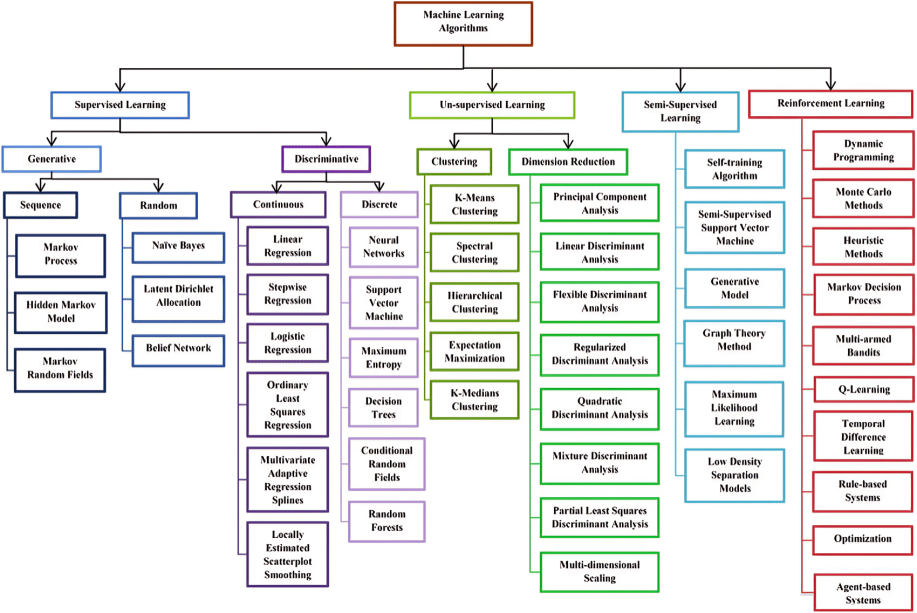
\includegraphics[width=1\textwidth,height=0.5\textheight]{img/Machine_Learning_ML_methods_taxonomy2.png}
     \caption{Techniques d'apprentissage automatique  \cite{sundararajan2021}}
     \label{fig:example2}
     \end{figure}

\subsection{types des techniques d'apprentissage automatique}   
\subsubsection{Apprentissage supervisé(Supervised Learning)}
Nous parlons des algorithmes qui ont besoin d'une supervision humaine qui alimente le dataset (les données à s'entrainer) avec des données de sortie , donc on a une connaissance préalable de ce que les valeurs de sortie pour nos échantillons devraient être \cite{apprentissage_supervise_definition}.Les modèles de l'apprentissage supervisé se composent de paires de données « d'entrée » et « de sortie », dans lesquelles la sortie est étiquetée avec la valeur souhaitée\cite{what_is_machine_learning}.
     \begin{figure}[htbp]
     \centering    
     \includegraphics[width=0.8\textwidth]{supervisé.png}
     \caption{déroulement standard d'un algorithme d'apprentissage supervisé  \cite{apprentissage_supervise_definition}}
     \label{fig:example3}
     \end{figure}

     
Au moyen d'un algorithme, le système compile l'ensemble de ces données d'entraînement et les met en corrélation (mesurer la relation entre une variable dépendante et une ou plusieurs variables indépendantes). Il commence alors à identifier des similarités, des différences et d'autres points de logique, jusqu'à ce qu'il puisse donner par lui-même la réponse à une question.

 
\textbf{Catégories des techniques de l'apprentissage supervisé :} il y a la classification donnée dans la figure 2.1 , et il existe aussi une classification qui est la plus connue dans plusieurs ressources : 

-\textbf{   a.Les algorithmes de régression :}des algorithmes qui cherchent à prédire une valeur continue, une quantité , tels que :
\begin{itemize}[label=$\bullet$]
\item Régression linéaire.
\item Régression polynomiale.
\item Régression Ridge.
\item Régression Lasso.
\item etc ...
\end{itemize}

-\textbf{   b.Les algorithmes de classification :}des algorithmes qui cherchent à prédire une classe/catégorie.
\begin{itemize}[label=$\bullet$]
\item Régression logistique.
\item Machine à vecteurs de support (SVM).
\item Forêt aléatoire.
\item Arbre de décision.
\item K-plus proches voisins (KNN).
\item Naïve Bayes.
\item etc ...
\end{itemize}

\textbf{Applications des techniques d'apprentissage supervisé :}
\begin{itemize}[label={*}]
\item Prédiction de la croissance démographique de la population
\item Détection des des spams ou du courrier indésirable.
\item prévisions météorologiques
\item Prédiction de la hausse/baisse de la valeur de la devise
\item etc ...
\end{itemize}

\vspace{2cm}

\subsubsection{Apprentissage non supervisé(Unsupervised Learning)}
Dans les modèles de cet apprentissage, aucune clé de réponse n'est fournie. La machine étudie les données d'entrée, dont la grande majorité sont non étiquetées et non structurées, et recherche des patterns et des corrélations entre les données pertinentes et accessibles.
Pour nous les humains , plus nous acquérons de l'expérience sur un élément ou un domaine, plus notre capacité à le catégoriser et à le repérer gagne en précision. Dans le cas des machines, « l'expérience » se traduit par le volume de données auxquelles elles ont accès\cite{what_is_machine_learning}. 

     \begin{figure}[htbp]
     \centering    
     \includegraphics[width=0.8\textwidth,height=0.3\textheight]{img/non_supervisé.png}
     \caption{déroulement standard d'un algorithme d'apprentissage non supervisé \cite{apprentissage_supervise_definition}}
     \label{fig:example4}
     \end{figure}



\textbf{Catégories des techniques de l'apprentissage non supervisé :}
 Il existe trois principales catégories d'algorithmes \cite{supervised_vs_unsupervised_learning}:
 
 \textbf{Clustering} : les données non étiquetées sont regroupées à l'aide de techniques de regroupement en fonction de leurs similitudes ou de leurs différences. Par exemple, si une équipe travaille sur la segmentation du marché, l'algorithme de clustering k-moyennes (k-means) attribuera des points de données similaires aux groupes qui représentent un ensemble de paramètres.

 \begin{figure}[htbp]
     \centering    
     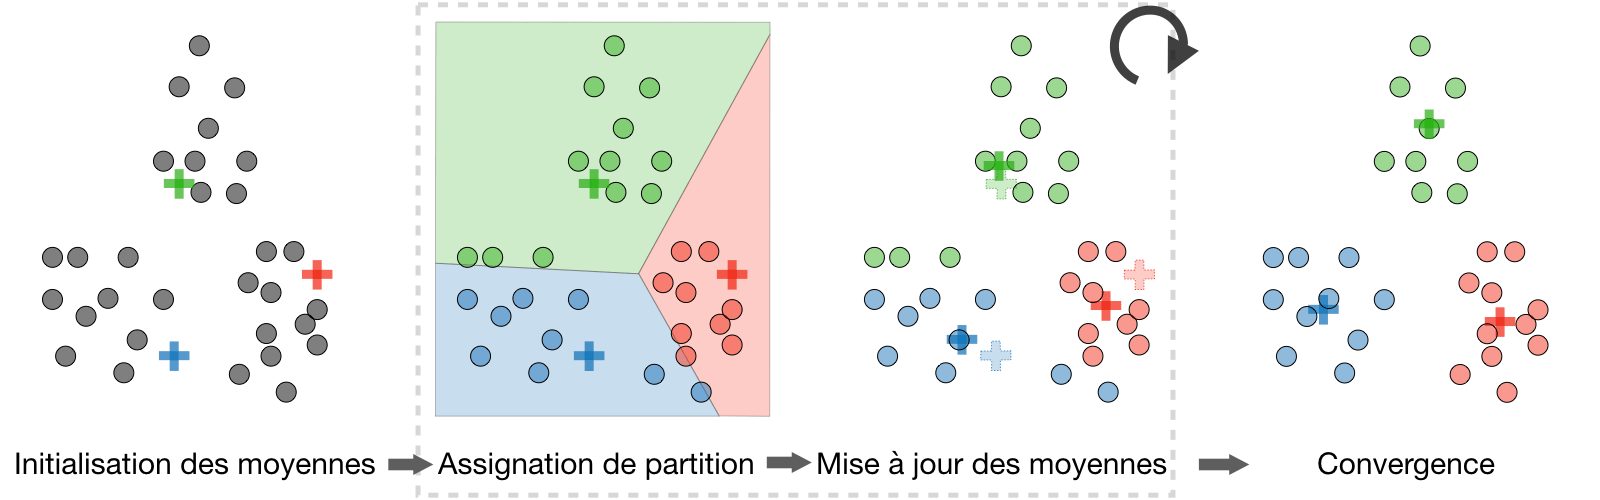
\includegraphics[width=0.9\textwidth,height=0.2\textheight]{k_means_fr.png}
     \caption{étapes de l'algorithme k-means \cite{pense_bete_apprentissage_non_supervise}}
     \label{fig:example5}
     \end{figure}


\textbf{Association} : cette catégorie est intéressante pour trouver des relations entre les variables d'un jeu de données. C'est la technique utilisée pour créer le message de type « les autres clients ont également consulté ». Elle est particulièrement adaptée aux moteurs de recommandation. 

\vspace{1cm}

\textbf{Réduction de la dimensionnalité} : il arrive qu'un jeu de données comporte un nombre de caractéristiques exceptionnellement élevé. La réduction de la dimensionnalité permet de réduire ce nombre sans compromettre l'intégrité des données. Il s'agit d'une technique couramment utilisée avant le traitement des données. Cela sert par exemple à supprimer le bruit d'une image pour améliorer sa qualité.


\begin{figure}[htbp]
     \centering    
     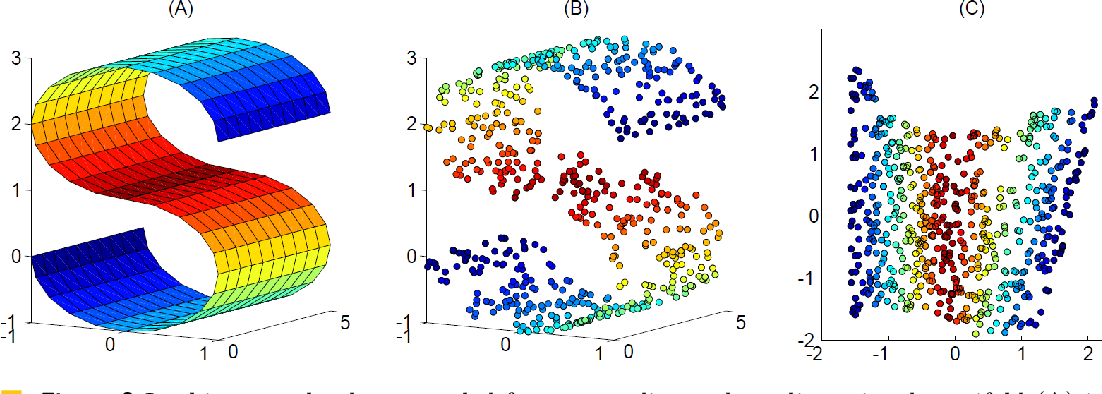
\includegraphics[width=0.8\textwidth]{réduction_de_dimensionalité.png}
     \caption{Exemple de réduction de dimensionalité (3D vers 2D) \cite{reduction_de_dimensionalite}}
     \label{fig:example6}
     \end{figure}

\vspace{1cm}

\textbf{Applications des techniques d'apprentissage non-supervisé :}
\begin{itemize}[label={*}]
\item La reconnaissance faciale.
\item L'analyse de séquences génétiques.
\item Les études de marché.
\item la cybersécurité.
\item etc ...
\end{itemize}

     \begin{figure}[htbp]
     \centering    
     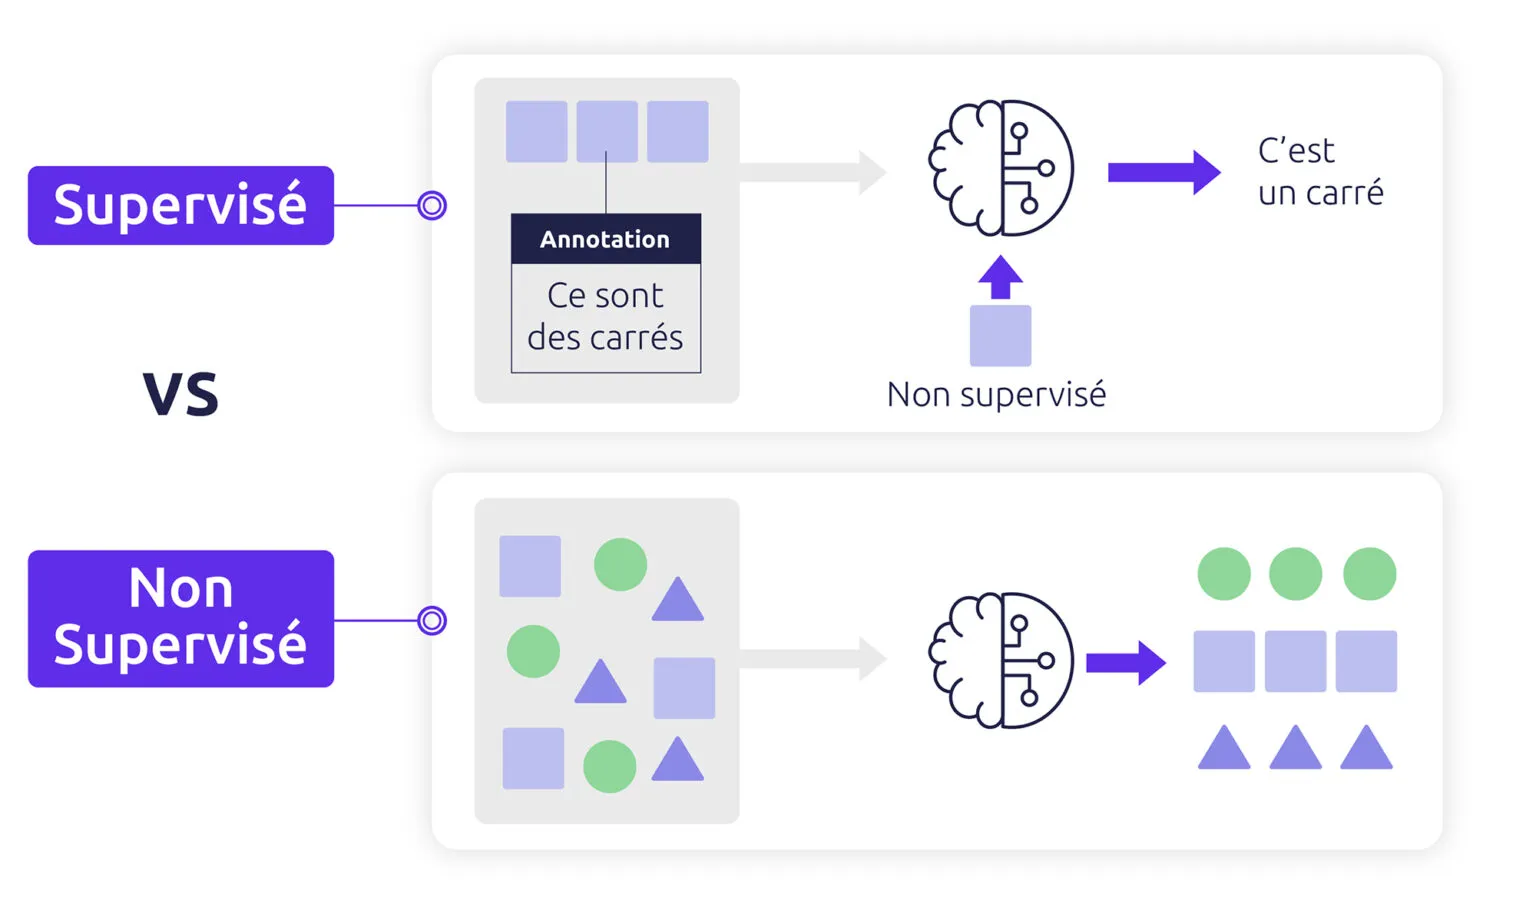
\includegraphics[width=0.7\textwidth,height=0.3\textheight]{img/non_supervisé_vs_supervisé.png}
     \caption{shéma montrant la différence majeur entre les algorithmes supervisés et non-supervisés \cite{non_supervisé_vs_supervisé}}
     \label{fig:example7}
     \end{figure}


\subsubsection{Apprentissage semi-supervisé(Semi-Supervised Learning) }
Dans cet apprentissage, toutes les données seraient structurées et étiquetées avant d'être placées dans un système. Mais comme ce n'est évidemment pas possible, l'apprentissage semi-supervisé constitue une solution envisageable lorsqu'on utilise de gros volumes de données brutes et non structurées. Ce type de modèle consiste à insérer de petites volumes de données étiquetées pour enrichir des ensembles de données non étiquetés. Un algorithme d'apprentissage semi-supervisé invite la machine à analyser les données étiquetées afin de déterminer des propriétés corrélatives qui pourraient être appliquées aux données non étiquetées.\cite{what_is_machine_learning}

\textbf{Applications des techniques d'apprentissage semi-supervisé \cite{what_is_machine_learning}:}
\begin{itemize}[label={*}]
\item L'analyse du discours et de la langue.
\item Les recherches médicales complexes.
\item Détection de fraude à un niveau général.
\item etc ...
\end{itemize}

\vspace{2cm}


\subsubsection{Apprentissage par renforcement (Reinforcement Learning)}
Il désigne l’ensemble des méthodes qui permettent à un agent(machine) d’apprendre à choisir quelle action prendre, et ceci de manière autonome .
Plongé dans un environnement donné, il apprend en recevant des récompenses ou des pénalités en fonction de ses actions. Au travers de son expérience, l’agent cherche à trouver la stratégie décisionnelle optimale qui puisse lui permettre de maximiser les récompenses accumulées au cours du temps.

     \begin{figure}[htbp]
     \centering    
     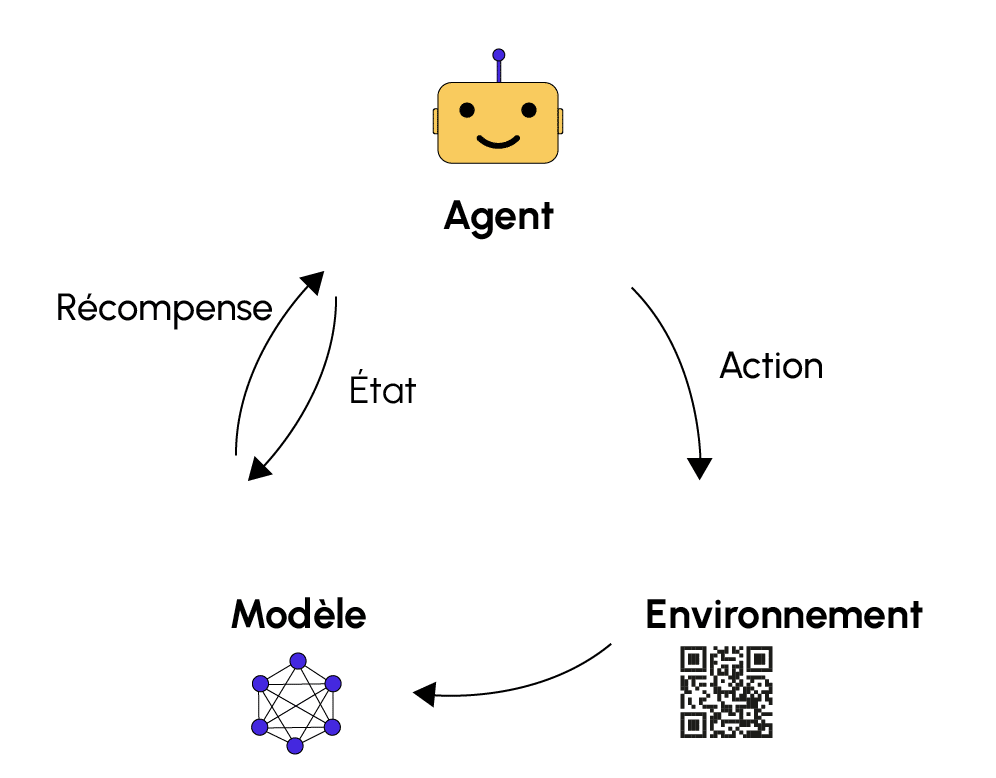
\includegraphics[width=0.7\textwidth,height=0.3\textheight]{img/reinforcement_learning.png}
     \caption{schéma résumant le processuss des algorithmes d'apprentissage par renforcement \cite{reinforcement_learning}}
     \label{fig:example8}
     \end{figure}

\vspace{1cm}     
\textbf{Techniques de l'apprentissage par renforcement :}
Il existe un certain nombre des méthodes les plus connues \cite{basics_of_reinforcement_learning} :
\begin{itemize}[label=$\bullet$]
\item \textbf{Q-learning} : un algorithme qui estime la valeur des paires état-action et met à jour de manière itérative les valeurs Q en fonction des récompenses observées. En apprenant une politique optimale directement à partir de l'expérience, Q-learning permet aux agents de prendre des décisions intelligentes
\item \textbf{Réseaux Q-profonds (DQN)} : Les réseaux Q profonds (DQN) combinent l'apprentissage par renforcement avec des réseaux de neurones profonds. Les DQN utilisent la puissance des architectures d'apprentissage profond pour se rapprocher des valeurs Q pour de grands espaces d'état-action. En utilisant des réseaux de neurones comme approximateurs de fonctions, les DQN peuvent gérer des environnements complexes et apprendre des représentations de grande dimension. Les DQN ont obtenu un succès remarquable dans différents domaines tels que jouer à des jeux Atari et contrôler des systèmes robotiques.
\item \textbf{Méthodes de gradients de politique} : Les méthodes de gradient de politique optimisent directement la politique en estimant les gradients des récompenses attendues par rapport aux paramètres de la politique. En mettant à jour de manière itérative la politique dans le sens de récompenses plus élevées, ces méthodes peuvent apprendre des politiques d’action complexes et continues. Les algorithmes de gradient de politique ont connu du succès dans des applications telles que le contrôle robotique et le traitement du langage naturel.
\item \textbf{Optimisation de la politique proximale (PPO)} : est un algorithme d'optimisation qui maintient un équilibre entre stabilité et efficacité des échantillons. PPO utilise une fonction d'objectif de substitution pour mettre à jour les paramètres de politique et garantir de petites mises à jour de politique afin de maintenir la stabilité. PPO a démontré des performances supérieures dans divers domaines tels que le jeu et la manipulation robotique.
\end{itemize}
\vspace{1cm}
Il existe d'autres méthodes qui ont été apparu avec l'avancement de ce type d'apprentissage , y compris l'apprentissage par renforcement multi-agents et le méta-apprentissage .

\textbf{Applications des techniques d'apprentissage par renforcement \cite{basics_of_reinforcement_learning}:}
\begin{itemize}[label={*}]
\item Robotique.
\item Véhicules autonomes.
\item Systèmes de recommandation.
\item etc ...
\end{itemize}


\newpage

\subsubsection{Différences entre les types d'apprentissage automatique} 
 \begin{figure}[htbp]
     \centering    
     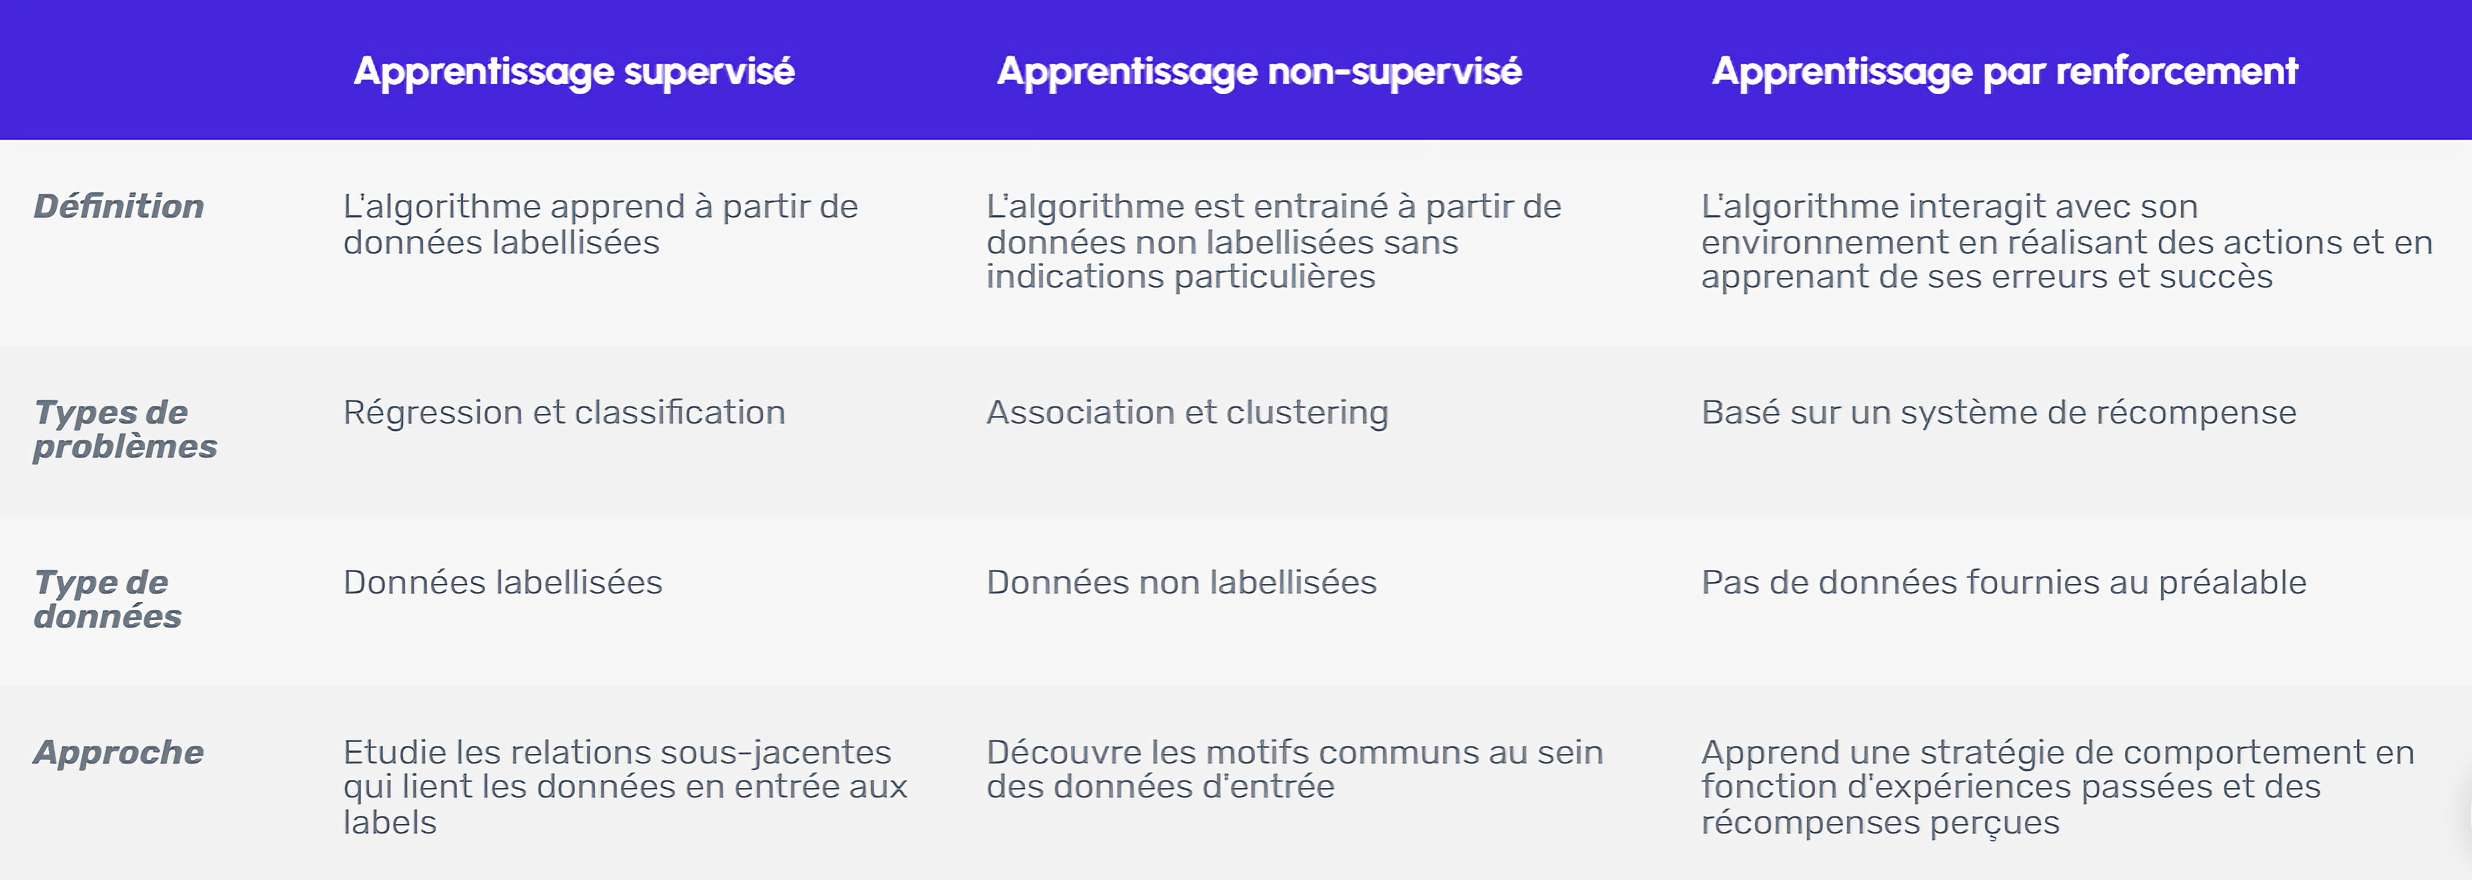
\includegraphics[width=1\textwidth,height=0.3\textheight]{différences.png}
     \caption{Différences entre les types d'apprentissage automatique \cite{reinforcement_learning}}
     \label{fig:example9}
     \end{figure}

 \vspace{3cm}    
 \section{Apprentissage profond}
  Le deep learning (Apprentissage profond) est une façon particulière de faire du machine learning (le deep learning(DL) est un sous-ensemble de techniques du machine learning), il se focalise sur des méthodes d'apprentissage automatique qui s'inspirent du fonctionnement du système nerveux de l'être humain.
 
 Contrairement à l'apprentissage automatique qui comprend des algorithmes de réseaux de neurones simples(nous allons clarifier cette notion après) , le deep learning comprend des techniques de réseaux de neurones avec des architectures beaucoup plus complexe (les notions "complexe" , "simple" et "couches" dans Table 1.1 vont être clarifiées après) .
 

\begin{center}
\begin{table}[htbp]
\begin{tabular}{|p{8cm}|p{8cm}|}
\hline
\textbf{NN du machine learning} & \textbf{NN du deep learning} \\ \hline
\hline
- Architecture simple (1-2 couches cachées) & - Architecture complexe (plusieurs couches cachées qui peuvent atteindre les centaines) \\
\hline
- Moins de puissance de calcul & - puissance de calcul trop importante \\
\hline
- Apprentissage souvent supervisé & - Apprentissage supervisé, non supervisé ou par renforcement \\
\hline
- Besoin d'une intervention humaine pour l'extraction des caractéristiques & - Pas besoin d'une intervention humaine \\
\hline
- traitement et observation des milliers de données & - traitement et observation d'une grande massivité de données (Big data)\\
\hline
- Applications: systèmes de recommandation , classification d'images, reconnaissance faciale, détection de fraude & - Applications: les applications du machine learning ,traitement du langage naturel, vision par ordinateur, traduction automatique \\
\hline
- utilisé par le data Analyst et data scientist & - utilisé par le data scientist seulement\\
\hline
\end{tabular}
\caption{Differences entre les réseaux de neurones du ML et du DL}
\end{table}
\end{center}


 \subsubsection{Principe des NN profonds}
 Ces algorithmes sont composés d'unités reliées entre elles qui vont s'entre activer (comme le cerveau humain) qu'on les appelle "neurones artificiels" , chaque neurone du réseau peut produire un effet sur ceux auxquels il est connecté. Ce qui presque commun entre toutes ces réseaux est que ces neurones sont organisés sous forme de couches (une couche d'entrée qui contient les neurones représentant les variables d'entrée , une couche de sortie qui contient le/les neurone(s) de sortie , et un certain nombre de couches cachées) reliées entre eux par la liaison entre le neurones des différentes couches . Toutefois, au lieu d'un signal électrique (comme dans le cerveau humain), le réseau de neurones attribue un certain poids à différents neurones .
    
    \begin{figure}[htbp]
     \centering  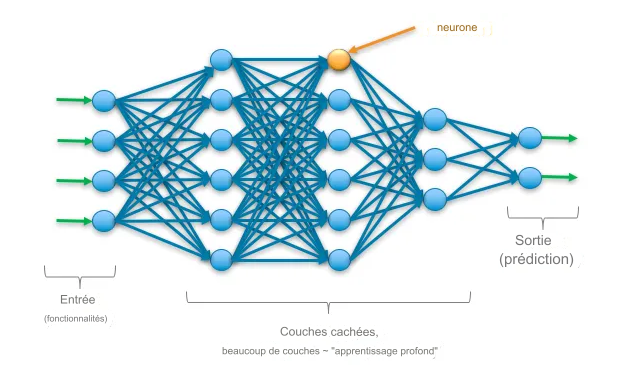
\includegraphics[width=0.8\textwidth,height=0.3\textheight]{img/NN.png}
     \caption{schéma d'un réseau de neurones profond (avec 3 couches cachées) }
     \label{fig:example10}
     \end{figure}
 \newpage
 
 \textbf{Modèles des réseaux de neurons profonds :} 
On ne peut jamais déterminer le nombre des architectures des NN créées jusqu'aujourd'hui (voir par exemple la figure~\ref{fig:NN_architectures} pour un aperçu des architectures de réseaux neuronaux.) , parce c'est une ensemble de modèles qui dépendent à plusieurs facteurs (prenons l'exemple des architectures citées dans la figure 1.10) , il suffit d'effectuer un petit changement dans un seul de ces facteurs et on va avoir un nouveau modèle . Parlant des facteurs , nous citons :

    \begin{itemize}[label=$\bullet$]
    \item \textbf{Architecture : }La topologie peut se différer beaucoup entre les architecture , dépandant des liasions entre les neurones quelque soit leurs couches ( comme c'est le cas dans les architectures citées dans la figure 1.10))
    
    \item \textbf{Taille du réseau :} Le nombre de neurones dans chaque couche peut être différent d'une couche à l'autre , sans parler de la différence de ce nombre entre les différentes architecture.
 
    \item \textbf{La profondeur du réseau :} nous pouvons avoir une architecture avec 3 couches cachées comme on peut trouver une architecture avec de centaines de couches cachées
    
    \item \textbf{Fonctions d’activation :} la fonction d'activation est une fonction mathématique appliquée à un signal en sortie d'un neurone artificiel . Elle va permettre le passage ou non de l’information si le seuil de stimulation est atteint. Concrètement, elle va avoir pour rôle de décider si on active ou non une réponse du neurone.
    Dans la figure 1.10 se mentionne les fonctions d'activation les plus connues , mais il y on a d'autres comme c'est plus détaillé dans \cite{nwankpa2018activation}
    
    \begin{figure}[htbp]
     \centering    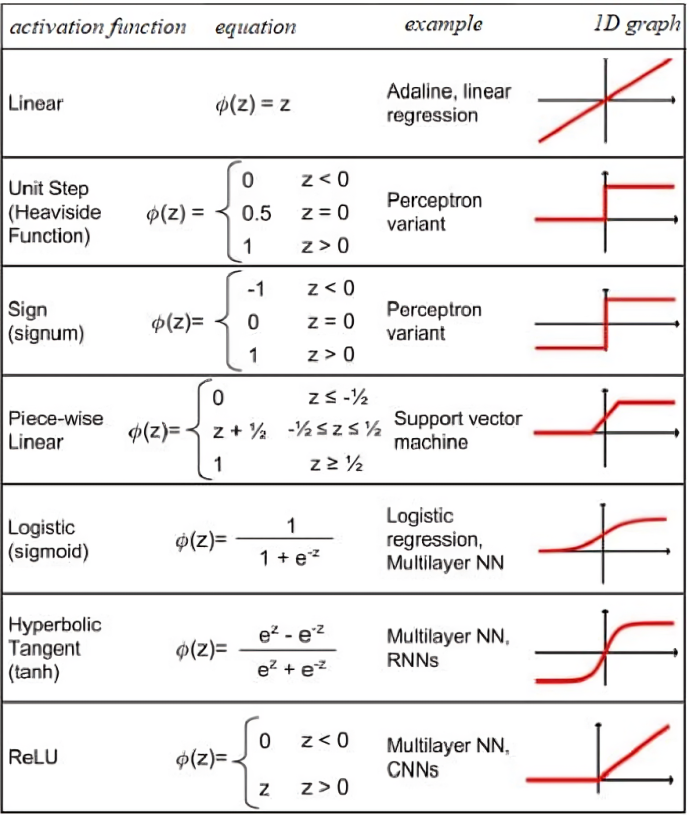
\includegraphics[width=0.65\textwidth,height=0.35\textheight]{activation_functions2.png}
     \caption{fonctions d'activtion dans un algorithme de NN profond\cite{activation_functions} }
     \label{fig:example11}
     \end{figure}
     \newpage
    \item \textbf{La pondération des connexions entre les neurones :} chaque connexion entre 2 neurones artificiels est pondérée par une valeur négative ou positive contrôlant l'impact des données communiquées entre ces unités . 
    \item \textbf{Valeur du biais:} c'est une valeur constante (ou un vecteur constant) ajoutée au produit des entrées et des poids dans un neurone artificiel afin d'affecter la sortie de la fonction d'activation.
    
    \begin{figure}[htbp]
     \centering  
     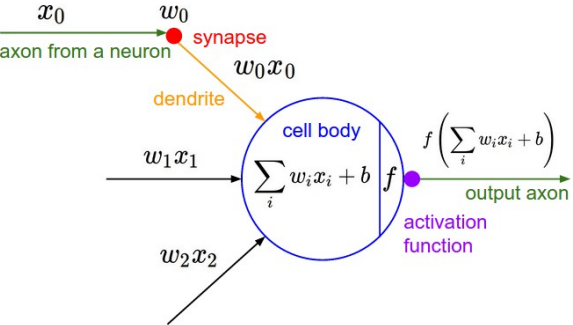
\includegraphics[width=0.55\textwidth,height=0.2\textheight]{neurone_detail.png}
     \caption{Schéma des opérations dans et entre les neurones artificiels\cite{neurone_detail} }
     \label{fig:example12}
     \end{figure}
    
    \item \textbf{Type de régularisation:}la régularisation comprend un ensemble de technique pour éviter le surapprentissage (overfitting) y compris :  \textbf{Normalisation ,dropout, régularisation L1 et L2 , et Early Stopping} 
    
    \item \textbf{Type de rétropropagation:} la rétropropagation est un ensemble de technique utilisées pour ajuster les poids des connexions entre les neurones , y compris \textbf{Rétropropagation avec Momentum , avec AdaGrad , avec Nesterov  gradient acceleré ,avec RMSProp , avec Adam , etc ... }
    
    \end{itemize}
    
    
   %  \begin{figure}
   %  \centering    
   %  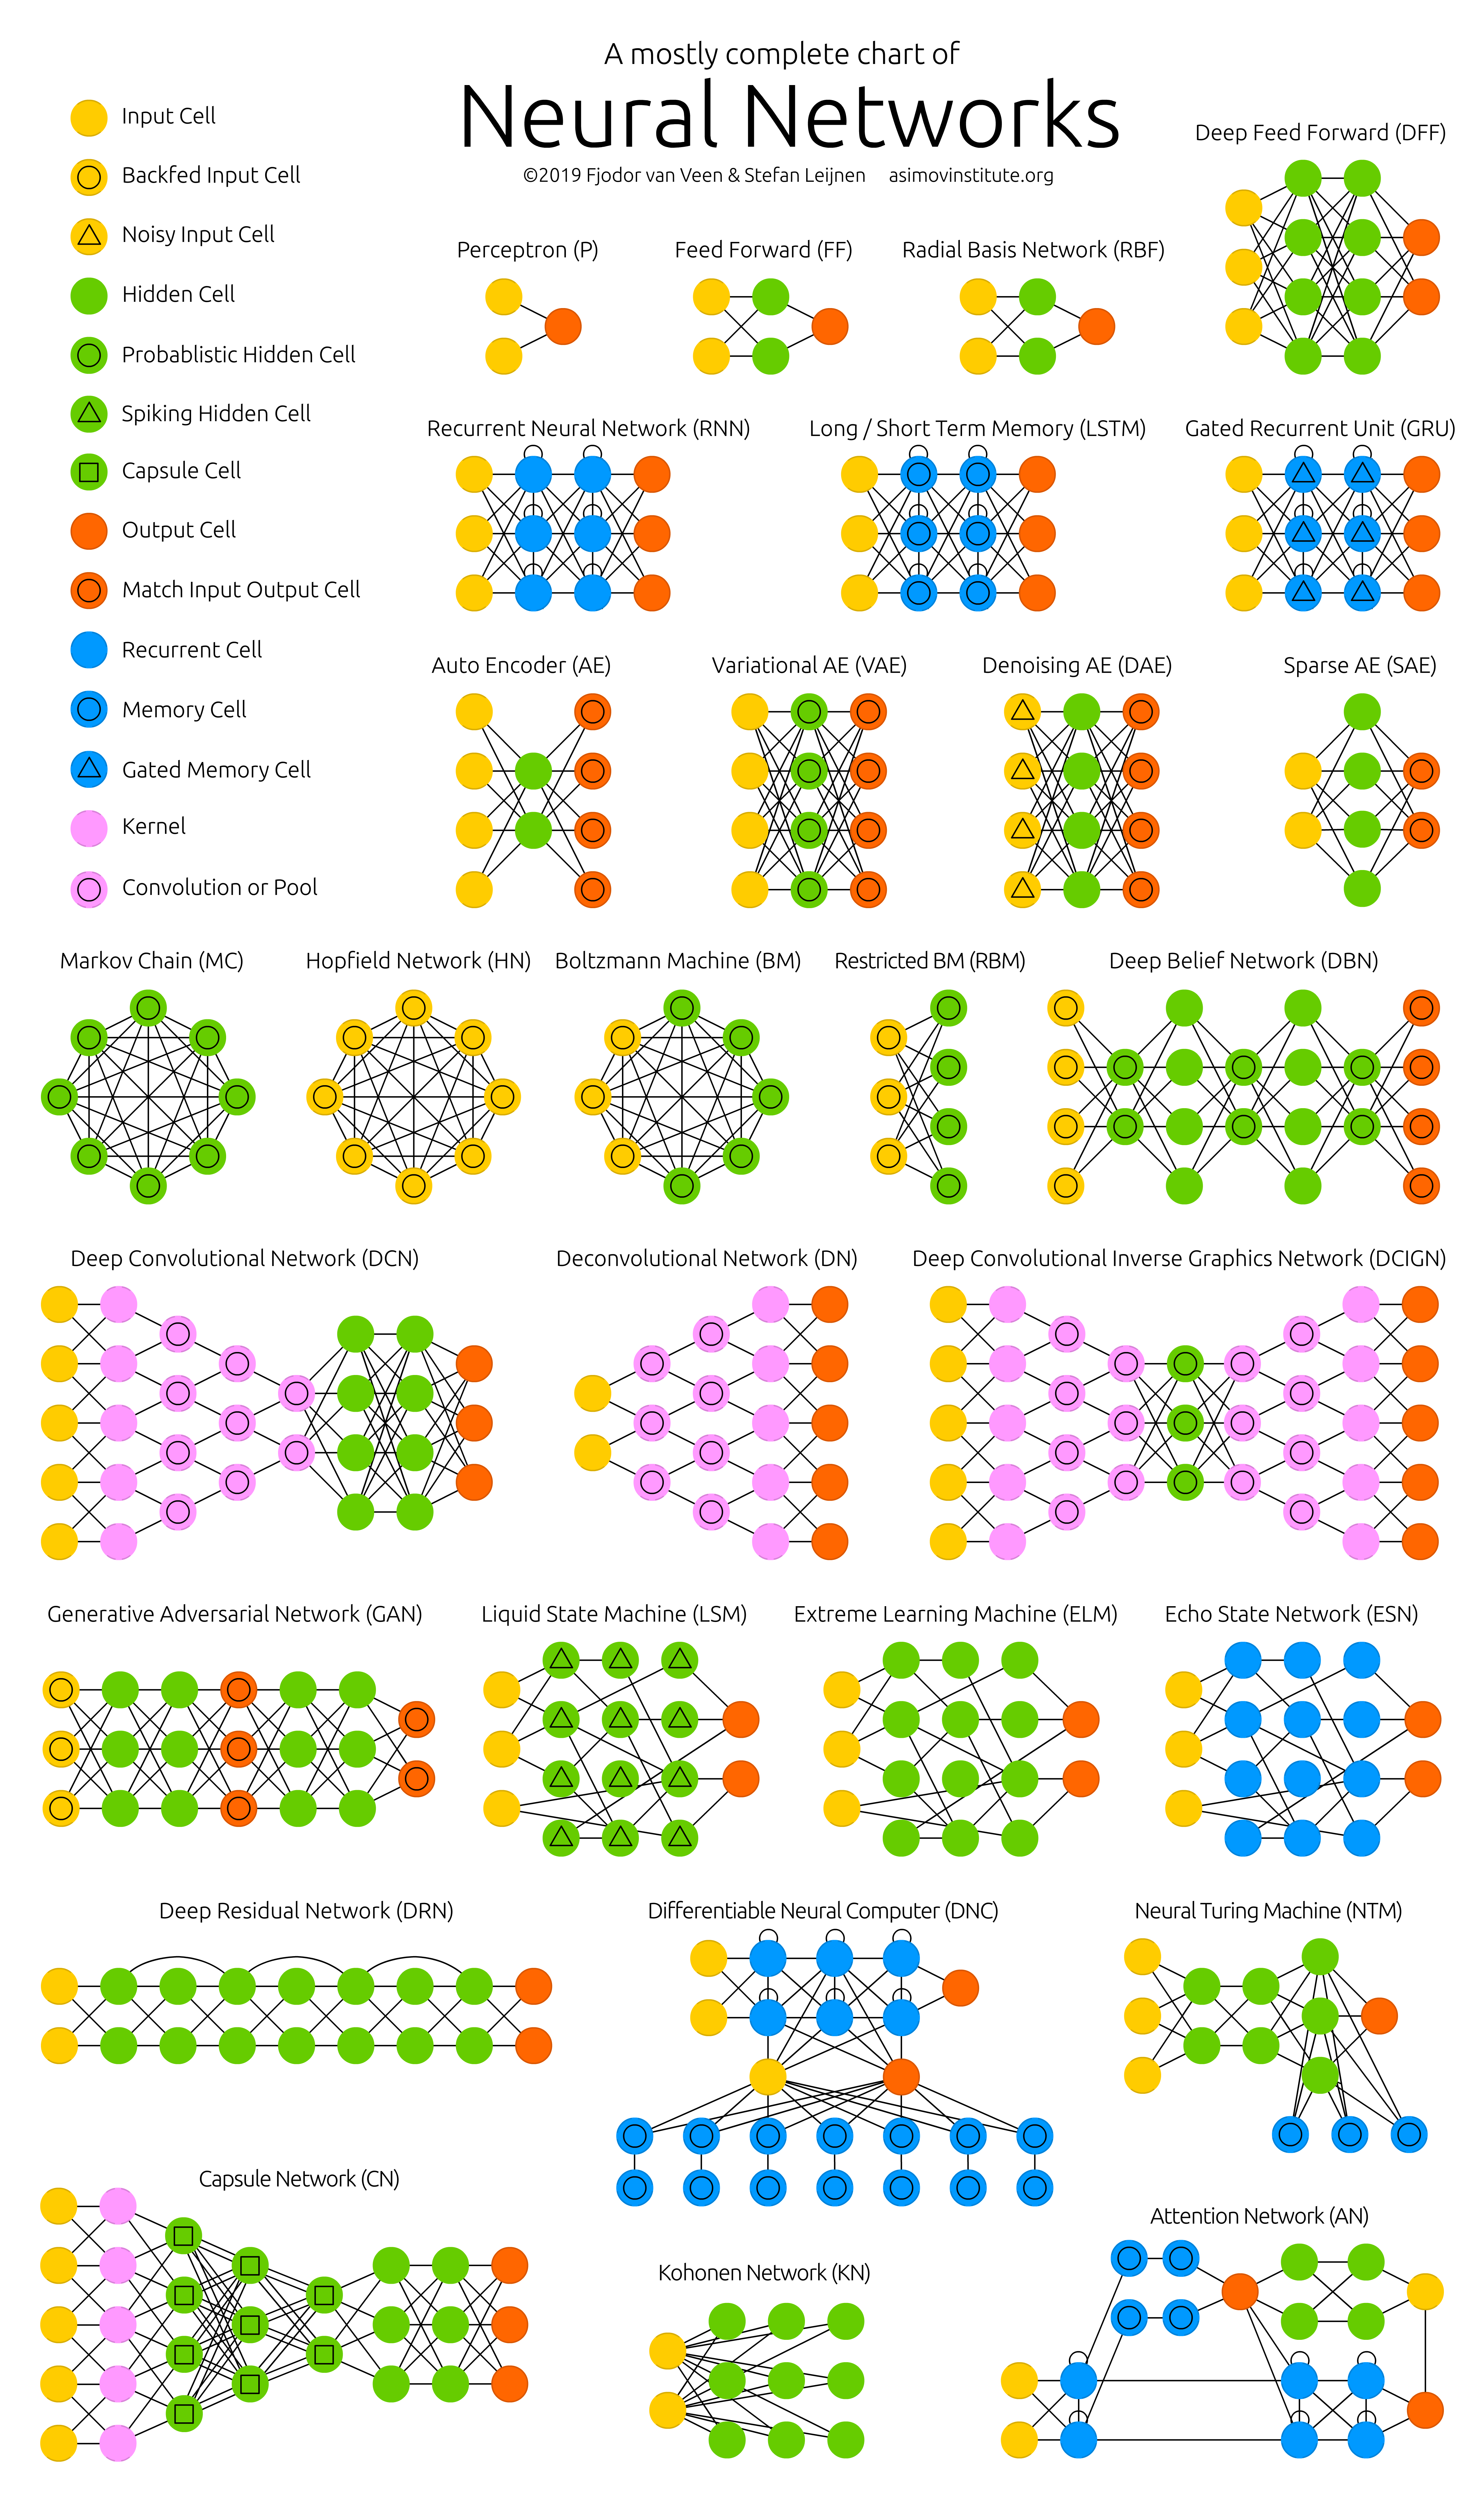
\includegraphics[width=1\textwidth,height=0.95\textheight]{NeuralNetworkZo19High.png}
   %  \caption{Un aperçu des architectures de réseaux neuronaux\cite{leijnen2020neural}}
   %  \label{fig:example13}
   %  \end{figure}



 \subsubsection{Types d'algorithmes d'apprentissage pronfond}
 Il existe différents types d'algorithmes , tel que \cite{algorithmes_deep_learning} :
 \begin{itemize}[label=$\bullet$]
\item \textbf{Réseaux neuronaux convolutifs (CNN) :}
les CNN (appelés aussi ConvNets) sont constitués d'une multitude de couches chargées de traiter et d'extraire les caractéristiques des données. De manière spécifique, les CNNs sont utilisés pour l'analyse et la détection d'objets.Donc , Ils peuvent donc servir dans le domaine vision ppar ordinateur (reconnaître des images satellites, traiter des images médicales, détecter des anomalies ou prédire des séries chronologiques, etc ...)

    \begin{figure}[htbp]
    \centering
    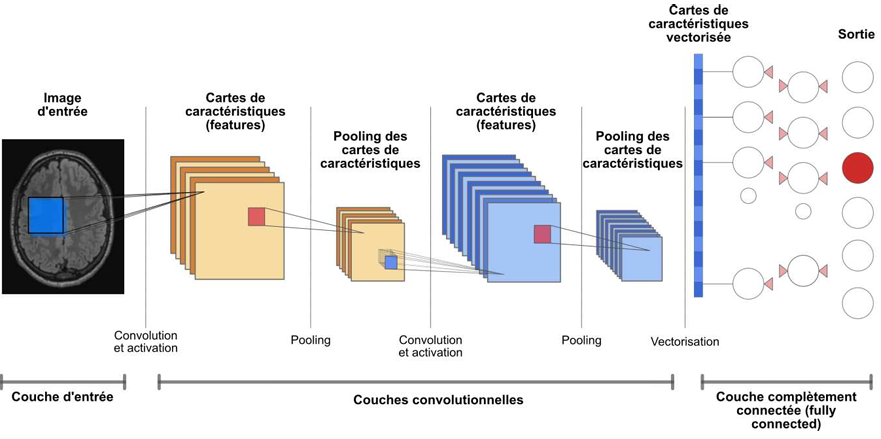
\includegraphics[width=0.6\textwidth,height=0.3\textheight]{CNN.png}
    \caption{Schéma général de principe de fonctionnement d'un réseau de neurones convolutifs \cite{fernandez_maloigne2019}.}
    \label{fig:example14}
    \end{figure}

\item \textbf{Réseaux neuronaux récurrents (RNN) :}
Les RNNs possèdent des connexions qui constituent des cycles dirigés. Cela permet aux sorties du LSTM (que nous allons le mentionner après) d'être exploitées comme entrées au niveau de la phase actuelle. Elle peut donc mémoriser les entrées précédentes à l'aide de sa mémoire interne. Dans la pratique, les RNN sont utilisés pour le sous-titrage d'images, le traitement du langage naturel et la traduction automatique.

    \begin{figure}[htbp]
    \centering
    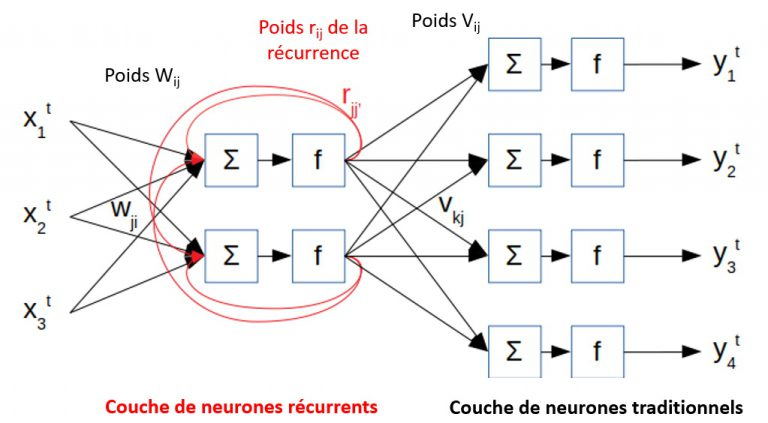
\includegraphics[width=0.4\textwidth,height=0.2\textheight]{RNN.jpg}
    \caption{Couche de neurones récurrents devant une couche de neurones traditionnels.
    \cite{LSTM}}
    \label{fig:example15}
     \end{figure}
     \newpage

 
\item \textbf{Réseaux de mémoire à long et court terme (LSTM) :}Les LSTM sont des dérivés de RNN. Ils peuvent apprendre et mémoriser des dépendances sur une longue durée. Les LSTM conservent ainsi les informations mémorisées sur le long terme. Ils sont particulièrement utiles pour prédire des séries chronologiques, car ils se rappellent des entrées précédentes. Outre ce cas d'utilisation, les LSTM sont également utilisés pour composer des notes de musique et reconnaître des voix.

    \begin{figure}[htbp]
    \centering
    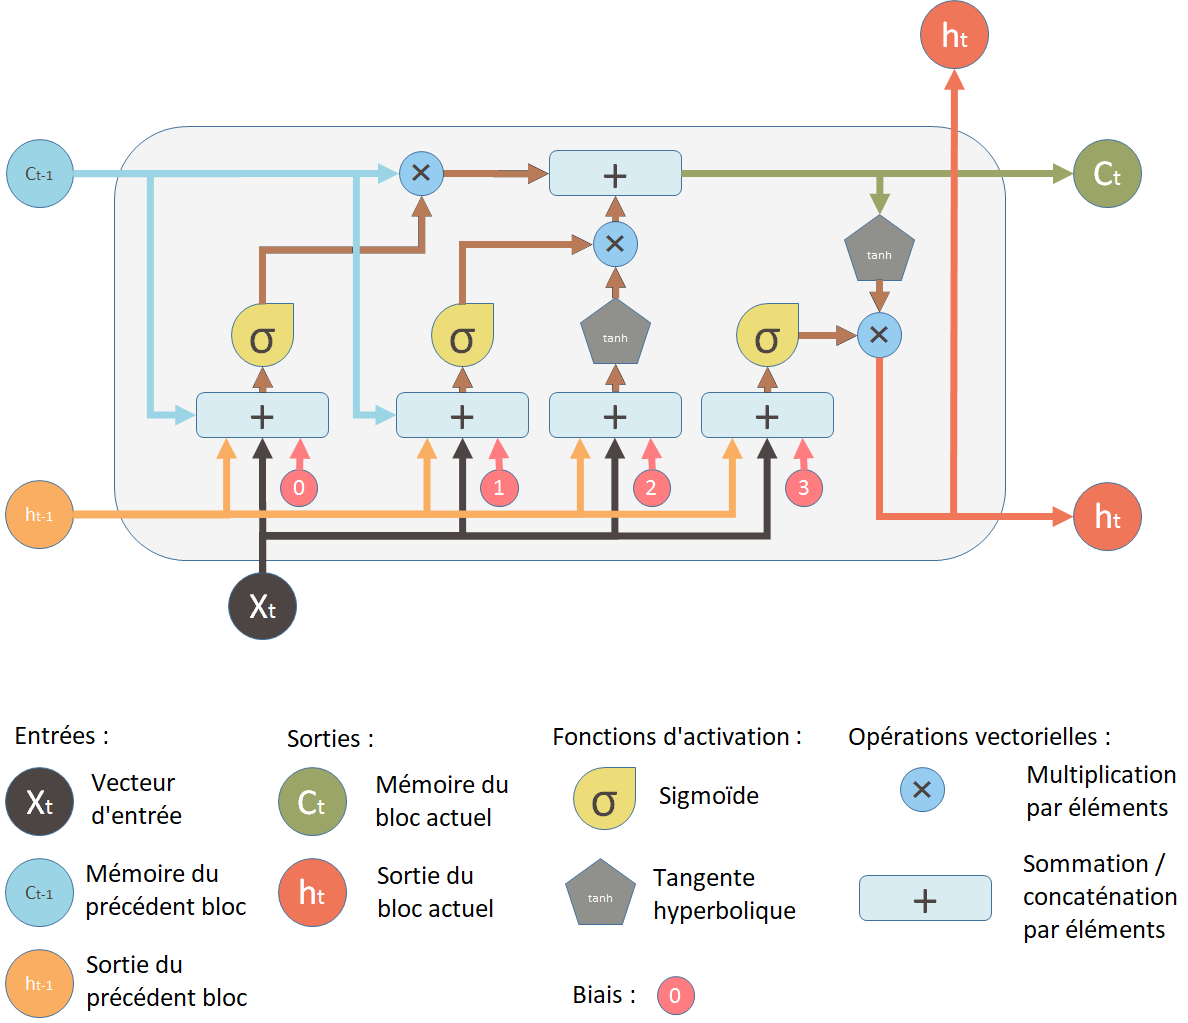
\includegraphics[width=0.6\textwidth,height=0.3\textheight]{img/LSTM.png}
    \caption{Schéma d'un exemple de réseau LSTM.
    \cite{LSTM}}
    \label{fig:example16}
    \end{figure}
     
\item \textbf{Réseaux adversariaux génératifs (GAN) :}
Les GAN créent de nouvelles instances de données qui s'apparentent aux données d'apprentissage profond. Ils possèdent deux principaux composants : un générateur et un discriminateur. Si le générateur apprend à produire des informations erronées, le discriminateur, quant à lui, apprend à exploiter ces fausses informations. Les GAN sont généralement utilisés par les créateurs de jeux vidéo pour améliorer les textures 2D.

    \begin{figure}[htbp]
    \centering
    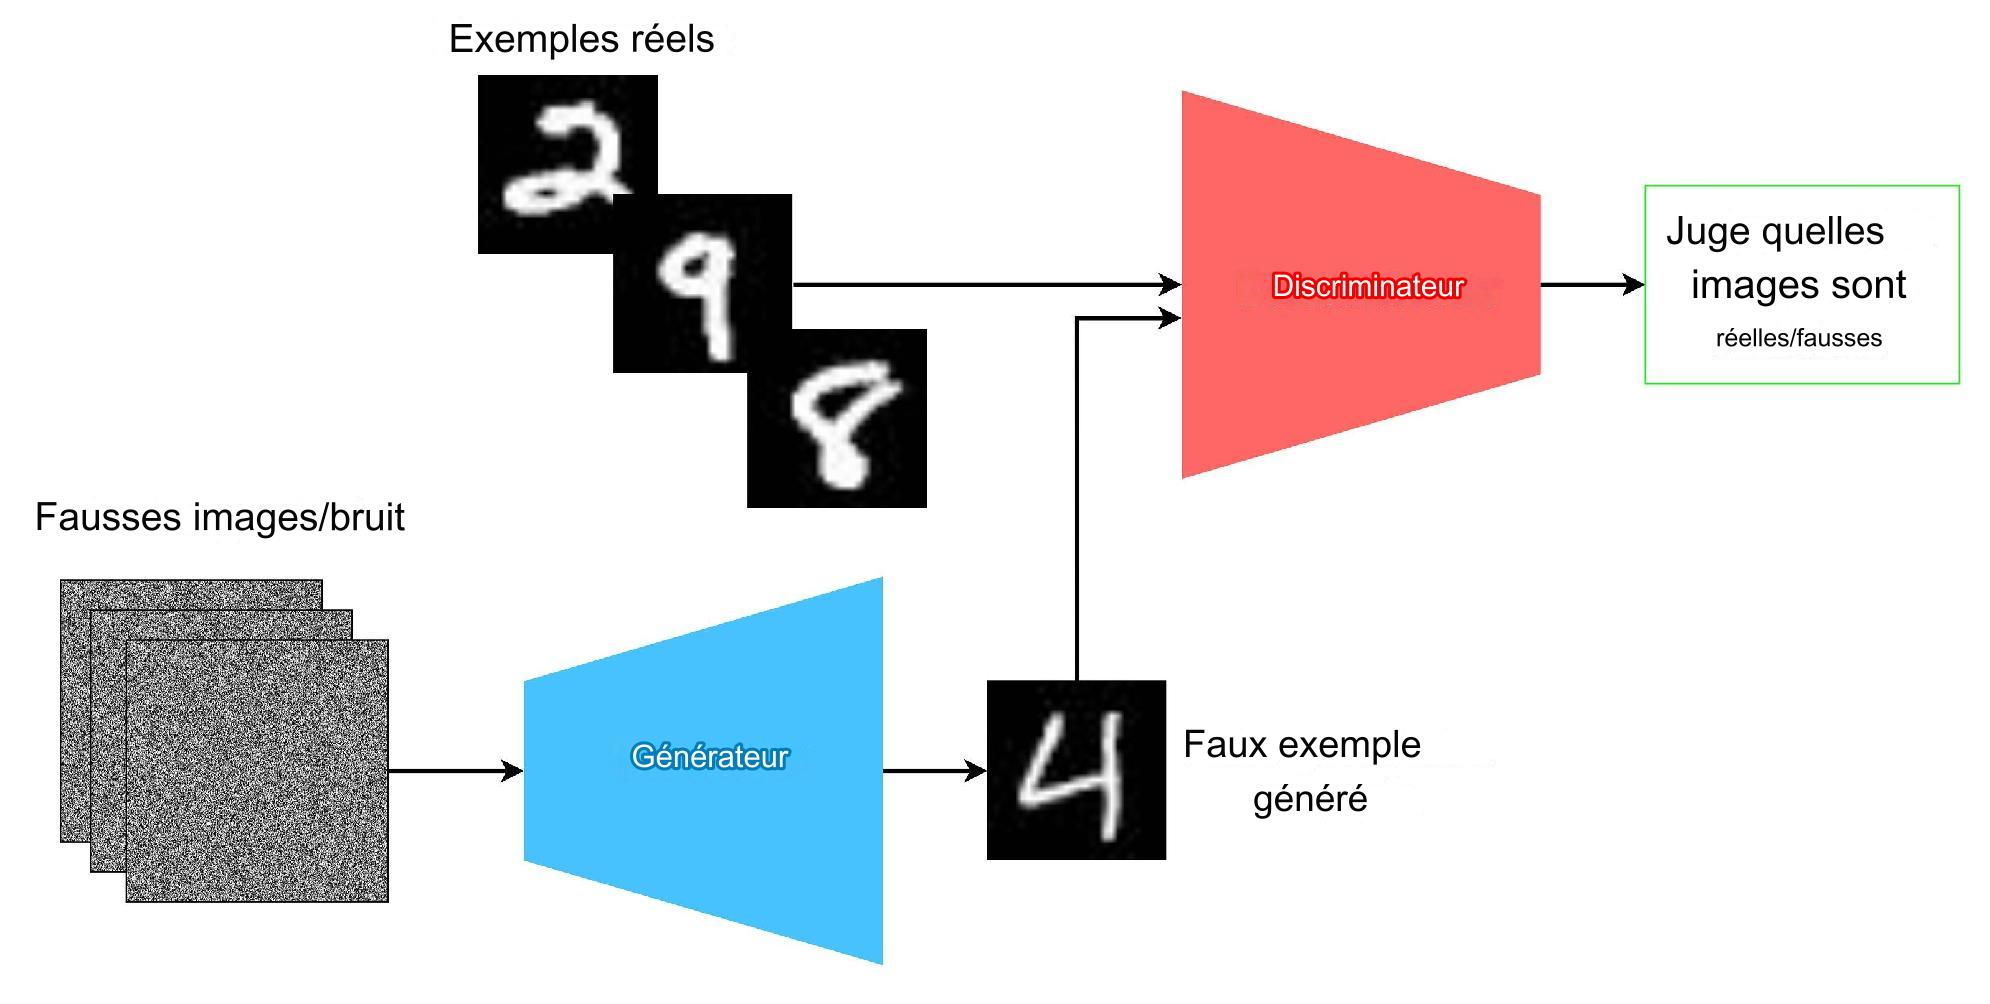
\includegraphics[width=0.9\textwidth,height=0.3\textheight]{img/GAN.jpg}
    \caption{Schéma decriptif du principe des GANs.
    \cite{generative_adversarial_networks_explained/}}
    \label{fig:example17}
    \end{figure}

\item \textbf{Machines de Boltzmann restreintes (RBM) :}
Ce sont des réseaux neuronaux stochastiques(avec des probabilités) constitués de deux couches : unités visibles et unités cachées. Ces réseaux artificiels sont capables d'apprendre en partant d'une distribution de probabilité sur un ensemble d'entrées. 
    
    \begin{figure}[htbp]
    \centering
    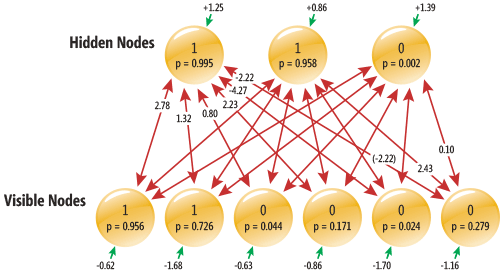
\includegraphics[width=0.6\textwidth,height=0.2\textheight]{img/RBM.png}
    \caption{Schéma d'un exemple de machines de Boltzmann restreintes.
    \cite{RBM}}
    \label{fig:example18}
    \end{figure}

Néanmoins, il est important de souligner que la liste d'algorithmes présentés ci-dessus n'est pas exhaustive. Il en existe d'autres types comme :
- les auto-encodeurs,
- les réseaux de croyance profonds (DBN),
les perceptrons multicouches (MLP).
- Les cartes auto-organisées (SOM) 
\end{itemize}


     
\subsection{Apprentisssage ensembliste}
Aussi appelé ensemble learning, c'est un ensemble de techniques qui combinent plusieurs algorithmes d’apprentissage automatique pour améliorer la précision des prédictions que celles obtenues avec un de ces algorithmes .

\subsubsection{Types des techniques d'apprentissage ensembliste} 
\begin{itemize}[label=$\bullet$] 

\item \textbf{Bagging (Bootstrap Aggregating)} :
Il consiste à entraîner plusieurs modèles ( du même type généralement ) sur des sous-ensembles aléatoires du jeu de données d’entraînement.
Chaque modèle est formé indépendamment, ce qui va réduir la variance et le surajustement (overfitting).
Les prédictions de ces modèles sont par la suite agrégées par vote majoritaire ou moyenne pour obtenir une prédiction finale plus robuste.
L’exemple le plus célèbre de bagging est l’algorithme Random Forest.

\item \textbf{Boosting} :
C'est un ensemble de modèles relativement faibles en séquence.
Chaque modèle est ajusté pour corriger les erreurs du modèle précédent. Les observations mal prédites (par les modèles précédents) reçoivent plus de poids, ce qui permet d’améliorer progressivement la performance globale.
Parmi les exemples populaires de boosting on trouve : \\ \textbf{AdaBoost} : Il ajuste de manière itérative le poids des observations en accordant plus d’importance à celles qui sont mal classées afin d'avoir un modèle fort qui est une combinaison de modèles relativement faibles .) \\
\textbf{Gradient Boosting} : Il optimise une fonction de perte en utilisant des gradients pour ajuster les prédictions du modèle.
Le gradient boosting est largement utilisé dans les compétitions de machine learning..

    \begin{figure}[htbp]
     \centering    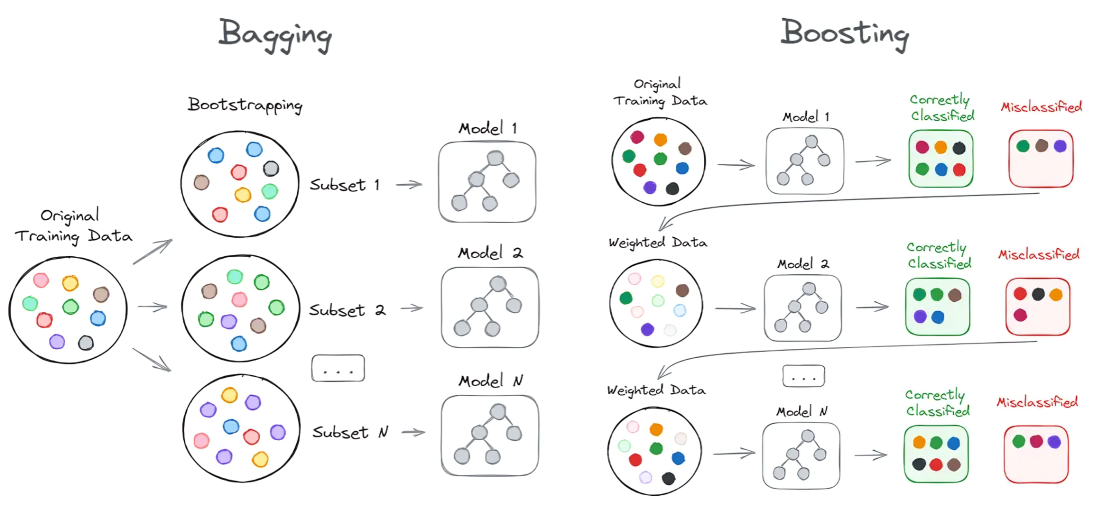
\includegraphics[width=0.7\textwidth,height=0.22\textheight]{img/baggingVSboosting.png}
     \caption{Schéma montrant la différence entre le bagging et le boosting \cite{sundararajan2021}}
     \label{fig:example19}
     \end{figure}
\item \textbf{Stacking} :
Le stacking (empilement) combine les prédictions de plusieurs modèles de base( après générer des prédictions sur les mêmes données d’entraînement.)
Par la suite, un modèle de méta-apprentissage (modèle de niveau supérieur) est utilisé pour combiner ces prédictions de manière optimale.
L'empilement permet d’exploiter les forces de différents types de modèles.

    \begin{figure}[htbp]
    \centering
    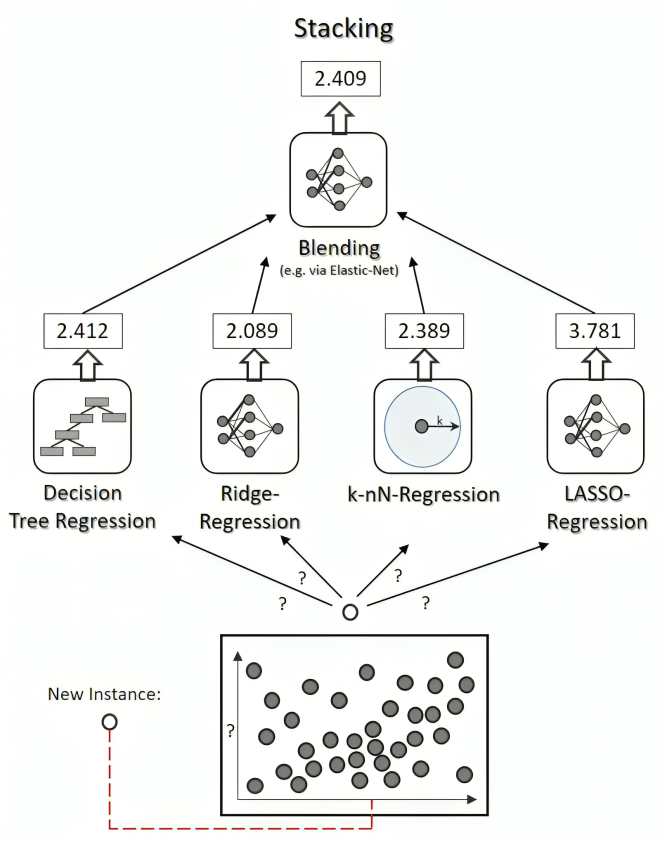
\includegraphics[width=0.55\textwidth,height=0.4\textheight]{stacking.png}
     \caption{Schéma d'un exemple du stacking\cite{stacking}}
     \label{fig:example20}
     \end{figure}
\newpage     
\item \textbf{Random Forest} :
Les forêts aléatoires sont des ensembles d’arbres de décision ,
chaque arbre est construit sur un sous-ensemble aléatoire du jeu de données . Les prédictions de chaque arbre sont agrégées par vote majoritaire, le truc qui va réduire l'overfitting et améliore la généralisation.

\begin{figure}[htbp]
     \centering    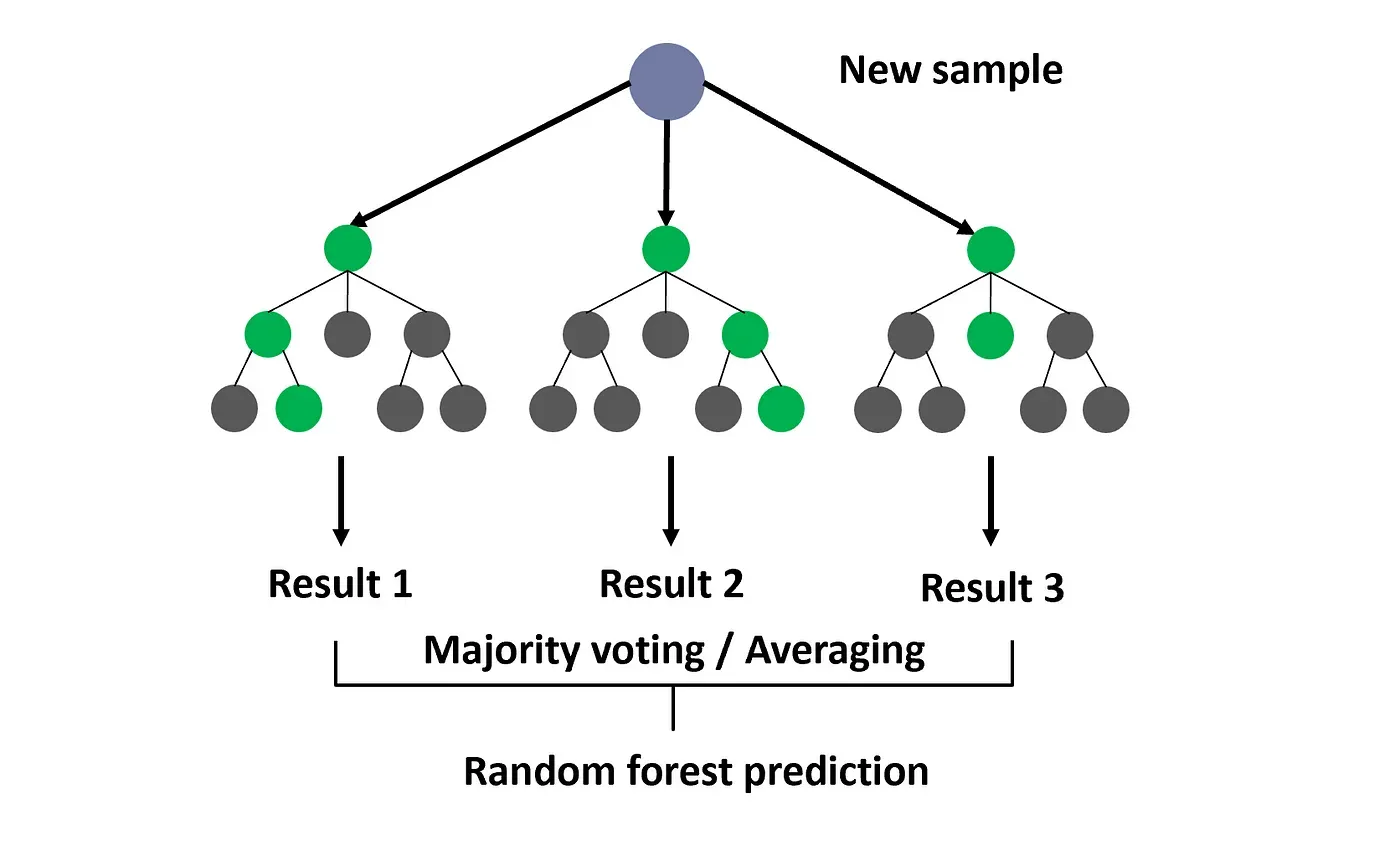
\includegraphics[width=0.6\textwidth,height=0.3\textheight]{img/random_forest.png}
     \caption{Schéma exemplaire d'une architecture d'ensembl learning de random forest \cite{random_forest}}
     \label{fig:example21}
     \end{figure}



\end{itemize}
% \subsection{Modèle CNN_différentes couches}
\subsection{Apprentissage basé transfert}
Connu aussi par "transfert learning" , c'est une famille de technique d’apprentissage automatique qui profite des connaissances acquises lors de la résolution d’un problème (donc on a un modèle existant déja entrainé qui nous a aidé à acquéir des connaissances prêtes) pour les appliquer à un problème similaire ou plus spécifique.


\subsubsection{Types de techniques de transfert learning}
\begin{itemize}[label=$\bullet$] 

\item \textbf{Transfert proche (inductif)} : Il se produit à l’intérieur d’un même domaine de connaissance ou d’une discipline spécifique
Exemple : utiliser un modèle pré-entraîné pour la classification d'images pour une nouvelle tâche de classification d'images.

\item \textbf{Transfert lointain (transductif)} : Il se produit entre des domaines très différents et c'est plus général où la tâche cible et la tâche source sont différentes concernant la distribution de données, mais partagent des similarités structurelles.
Exemple : utiliser un modèle pré-entraîné pour la reconnaissance d'objets pour une nouvelle tâche de détection d'anomalies.

\end{itemize}



\subsection{Mesures d'évaluation des modèles}
L’évaluation des modèles d’apprentissage automatique profond est nécessaire pour savoir leurs performances et leurs précision à résulter la bonne prédiction. Alors,  nous utilisons des mesures quantitatives  qui fournissent un aperçu des performances du modèle et aident à comparer différents modèles ou algorithmes. On cite par exemple \cite{important_model_evaluation_error_metrics} \cite{classification_metrics_matrice_de_confusion} \cite{confusion_matrix_accuracy_recall_precision_false_positive_rate_and_f_scores_explained}:
\begin{itemize}[label=$\bullet$] 
\item \textbf{Matrice de confusion} : Elle résume les prédictions du modèle sur lequel s’appuient toutes les métriques de classification que nous allons citer : accuracy, F1-score, courbe ROC, Précision , Rappel ...etc en determinant les vrais positifs, les vrais négatifs, les faux positifs et les faux négatifs tels que :\\
\textbf{Vrai positif(TP)} : vous aviez prédit du positif, et c’est vrai.\\
\textbf{Vrai négatif(TN)} : vous avez prédit un résultat négatif, et c'est vrai.\\
\textbf{Faux positif(FP)(Erreur de type 1)} : vous avez prédit un résultat positif et c'est faux, en réalité c'est négatif.\\
\textbf{Faux négatif(FN)(Erreur de type 2)} : vous avez prédit un résultat négatif et c'est faux, en réalité c'est positif.\\
    \begin{figure}[htbp]
    \centering
    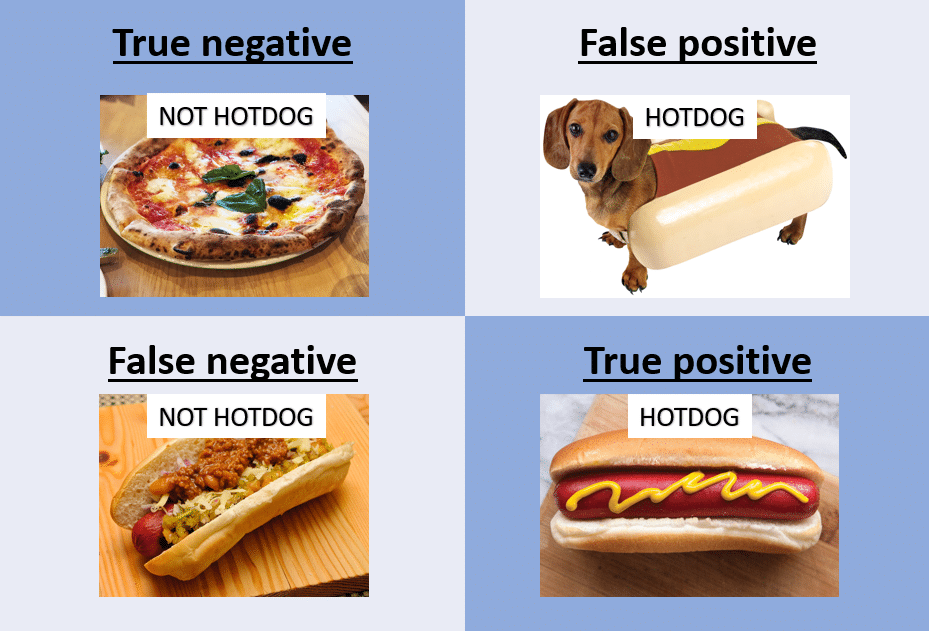
\includegraphics[width=0.5\textwidth,height=0.25\textheight]{matrice_confusion_elements.png}
    \caption{Illustration des éléments du matrice de confusion par images\cite{confusion_matrix_accuracy_recall_precision_false_positive_rate_and_f_scores_explained}}
    \label{fig:example22}
    \end{figure}
\item \textbf{Précision (Accuracy)} : Elle mesure le taux de prédictions correctes par rapport au nombre total d’échantillons positives .
\begin{equation}
\text{Precision} = \frac{\text{TP}}{\text{TP} + \text{FP}}
\end{equation}
\item \textbf{Rappel (Recall)} : Il évalue la capacité du modèle à détecter tous les exemples positifs. Donc , il correspond au taux d’individus positifs détectés par le modèle.
\begin{equation}
\text{Rappel} = \frac{\text{TP}}{\text{TP} + \text{FN}}
\end{equation}
    \begin{figure}[htbp]
    \centering
    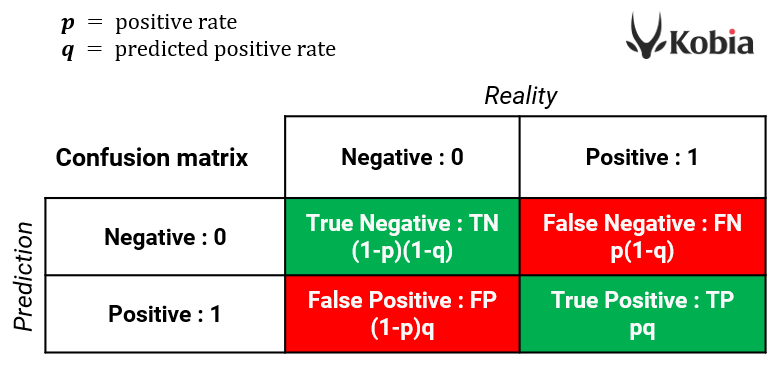
\includegraphics[width=0.7\textwidth,height=0.3\textheight]{calculs.png}
    \caption{Calculs des éléments du matrice de confusion\cite{classification_metrics_matrice_de_confusion}}
    \label{fig:example23}
    \end{figure}
\begin{align*}
p &= \frac{\text{FN}}{\text{TP} + \text{FN}} & ET&&
q &= \frac{\text{FP}}{\text{TP} + \text{FN}}
\end{align*}



\item \textbf{F1-mesure (F1-score)} : L’harmonique entre la précision et le rappel. Il combine ces deux mesures en une seule valeur, c'est utile lorsque nous souhaitons équilibrer les performances.
\begin{equation}
\text{F1-score} = \frac{2 \times \text{Precision} \times \text{Rappel}}{\text{Precision} + \text{Rappel}}
\end{equation} \\
Meme si nous voulons orienter l'évaluation selon un de ces deux mesures , un facteur beta est intégré comme la montre l'équation (1.4) tel que:\\ *beta < 1 : évaluation axée sur la précision\\
*beta > 1 : évaluation orientée rappel\\
\begin{equation}
F = (1 + \beta^2) \cdot \frac{\text{precision} \cdot \text{recall}}{\text{precision} - \beta^2 + \text{recall}}
\end{equation}

\item \textbf{Courbe ROC (Receiver Operating Characteristic)} : Elle représente la relation entre le taux de vrais positifs et le taux de faux positifs à différents seuils de classification. Nous allons calculer une métrique qui résume la performance globale du modèle : l’AUC (Area Under Cvover) , tel que : \\

- AUC = 0,5: Le modèle est équivalent à un tirage au sort (aléatoire). \\
- 0,5 < AUC < 1: Ce modèle est meilleur qu'un tirage au sort. \\
- AUC = 1: Le modèle est parfait (que de bonnes prédictions).

Si on prend AUC = 0.75 , cela signifie que la zone au dessous de la courbe (qui est réprésenté en rouge dans la figure 1.22) représente 75\% de la totalité du diagramme .
    \begin{figure}[htbp]
    \centering
    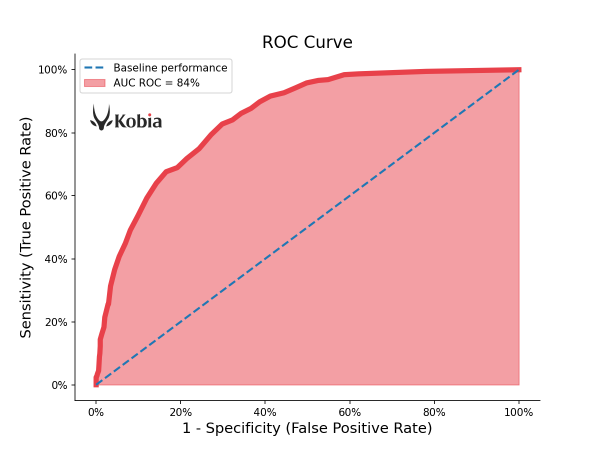
\includegraphics[width=0.7\textwidth,height=0.3\textheight]{AUC_ROC_application.png}
    \caption{Exemple d'une courbe ROC}\cite{classification_metrics_auc_roc}
    \label{fig:example24}
    \end{figure}
    \\
    tel que les facteurs nécessaires pour résulter cette courbe sont calculés de la manière suivante : \\
    \begin{figure}[htbp]
    \centering
    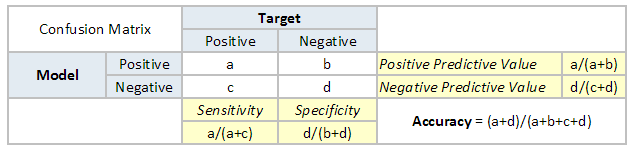
\includegraphics[width=0.8\textwidth,height=0.2\textheight]{ROC_facteurs.png}
    \caption{Calculs des facteurs du courbe AUC ROC\cite{important_model_evaluation_error_metrics}}
    \label{fig:example25}
    \end{figure}

    
\item \textbf{Perte (Loss)} : C'est une mesure utilisée pendant l’entraînement du modèle. Des fonctions de perte telles que l’entropie croisée binaire ou l’erreur quadratique moyenne sont couramment utilisées.


\item \textbf{Erreur quadratique moyenne}
C'est la moyenne des carrés des différences entre les prédictions du modèle et les valeurs réelles. Il existe aussi l'erreur logarithmique quadratique moyenne , les deux sont utilisées dans les modèles de régression.

\item \textbf{Entropie croisée (Cross-entropy)}
Dans les tâches de classification, nous traitons des prédictions de probabilités, ce qui signifie que la sortie d'un réseau neuronal doit être comprise entre zéro et un. Une fonction de perte capable de mesurer l'erreur entre une probabilité prédite et l'étiquette qui représente la classe réelle est appelée fonction de perte d'entropie croisée.
\begin{figure}[htbp]
    \centering
    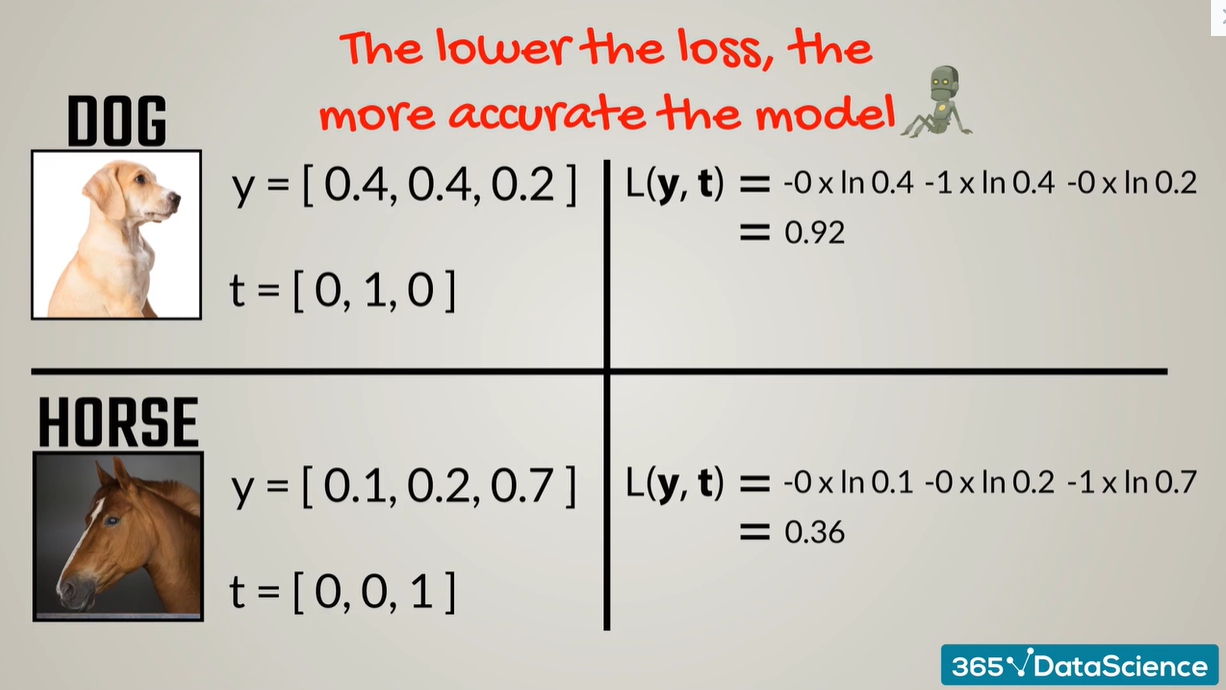
\includegraphics[width=0.6\textwidth,height=0.2\textheight]{cross_entropy_example.png}
    \caption{Exemple illustratif du déroulement de la fonction de perte "entropie croisée"\cite{cross_entropy_loss}}
    \label{fig:example26}
    \end{figure}
Une chose importante dont nous devons discuter avant de continuer avec l'entropie croisée est de savoir à quoi ressemble exactement le vecteur de vérité terrain dans le cas d'un problème de classification.

Le vecteur d'étiquette t est codé soit zéro soit un (soit le modèle a prédit l'objet/classe i (1) ou non(0) ).

La prédiction y peut cependant prendre des valeurs continues comprises entre zéro et un , car ils sont des probabilités que l'élément d'entrée soit de tel classe (pour chaque classe) .

Étant donné le vecteur de prédiction Y et le vecteur de vérité terrain Ŷ, vous pouvez calculer la perte d'entropie croisée entre ces deux vecteurs comme suit :

    \begin{figure}[htbp]
    \centering
    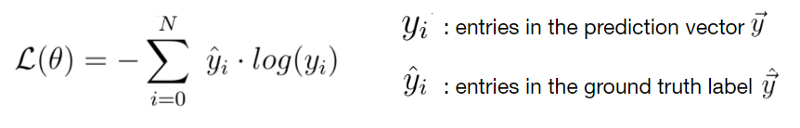
\includegraphics[width=0.5\textwidth,height=0.05\textheight]{loss_functions.png}
    \caption{Fonction de perte "Entropie croisée"\cite{loss_functions}}
    \label{fig:example27}
    \end{figure}


\item \textbf{R-carré/R-carré ajusté}
C'est une métrique statistique utilisée pour évaluer la qualité d'ajustement d'un modèle de régression.
\end{itemize}
\subsection{Conclusion}
En conclusion , la globalité des techniques de l'intelligence artificielle (que ça soit de l'IA ou le machine learning ou le deep learning) ont réussi à résoudre n'importe sorte de problème , simple ou compliqué
\chapter{Détection de la somnolence et l'hypovigilance en utilisant l'apprentissage profond}
\markboth{Détection de la somnolence et l'hypovigilance en utilisant l'apprentissage profond}{}


%-------------------
%-------------------
%-------------------

\section{Inroduction}
Les accidents de la route représentent une sérieuse menace pour la vie humaine, entraînant des pertes matérielles et humaines considérables, notamment en Algérie.
En 2022, les routes algériennes ont enregistré 22 980 accidents, causant 3 409 décès et 30 479 blessés\cite{AtlasMagasine2}, des chiffres alarmants qui montrent une tendance à la hausse constante.

Suite à des recherches et enquêtes menées par la DNSR, il a été établi que la somnolence est l'une des principales causes des accidents de la route. Selon la dernière étude du CNPSR en 2016 (DNSR avant) un tiers des accidents de la route en Algérie sont dus à la somnolence au volant. Cette situation a suscité des appels à classer les troubles du sommeil dans la même catégorie que les stupéfiants et l'alcool en raison de leur dangerosité\cite{autobip}.

En effet, sur les 10 accidents de la route enregistrés au cours des dix premiers mois de 2016, 2 500 ont été attribués à la somnolence au volant\cite{autobip}.

\section{Contexte et importance du problème}
La lutte contre la somnolence au volant revêt une importance cruciale, étant donné le nombre considérable d'accidents qu'elle entraîne, ainsi que les dégâts matériels et les pertes humaines qu'elle engendre. Selon des données fournies exclusivement pour le secteur de la Gendarmerie à la délégation nationale à la sécurité routière, le nombre d'accidents causés par la somnolence est en constante augmentation, comme le montre la \hyperlink{fig0} {figure}. Cette problématique est désormais classée dans la même catégorie que les stupéfiants et l’alcool en raison de sa dangerosité, non seulement en Algérie, mais à l’échelle mondiale. Par exemple en France, une étude de l'ASF en 2016 a identifié la somnolence au volant comme l’un des principaux facteurs de mortalité routière, comme illustré dans la \hyperlink{fig1} {figure 2}. Cette constatation démontre clairement que la détection de la somnolence a un impact potentiel sur la sécurité routière, où elle peut sauver des milliers de vies en restant vigilants et en s’arrêtant dès les premiers signes de fatigue, contribuant ainsi à réduire les risques d’accidents sur les routes en identifiant les signes de fatigue, ce qui permet de prendre des mesures pour éviter de conduire dans cet état dangereux.
\begin{figure}[H]
\hypertarget{fig0}{}
    \centering
    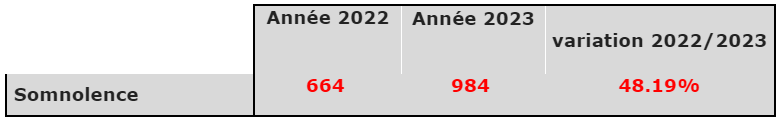
\includegraphics{img/accidents.png}
    \caption{ accidents corporels de la route causées par la somnolence}
    \label{fig:enter-label}
\end{figure}
\begin{figure}[H]
\hypertarget{fig1}{}
    \centering
    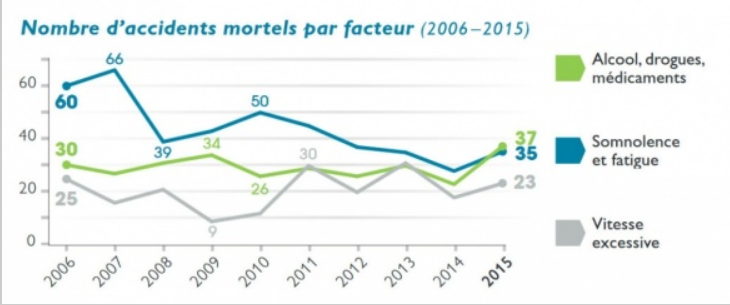
\includegraphics[]{img/frn.png}
    \caption{nombre d'accidents mortels par facture 2006-2015}
    
\end{figure}
Afin de mettre en place des mesures préventives efficaces, des systèmes de détection de la somnolence ont été développés. Ces systèmes ont pour objectif d'avertir les conducteurs avant que leur niveau de somnolence ne devienne critique, permettant ainsi de prévenir les accidents liés à ce phénomène. Néanmoins, la détection de la somnolence reste un défi majeur pour les chercheurs. Bien que de nombreux systèmes et solutions aient été développés, leur efficacité et leur fiabilité doivent encore être améliorées pour garantir une détection précise et prévenir efficacement les accidents.

\section{Somnolence au volant}
\subsection{La somnolence}
La somnolence, caractérisée par la tendance à s'endormir lorsque l'on souhaite rester éveillé, constitue l'un des symptômes les plus courants et significatifs signalés par les patients adressés à un spécialiste du sommeil. Ce phénomène est omniprésent et peut être le signe de diverses pathologies médicales, psychiatriques et troubles primaires du sommeil. Cependant, la somnolence est également un aspect physiologique, survenant au moins une fois par jour et pouvant être ressentie par tout individu dans des situations particulières\cite{haba2011somnolence}. Elle se manifeste souvent par des signes tels que des bâillements fréquents, une vision floue, des difficultés de concentration et une sensation de lourdeur dans les paupières. Plusieurs facteurs sous-jacents contribuent à cette sensation de somnolence. En conduisant, la somnolence peut conduire à des micro-sommeils, qui sont des périodes de sommeil de courte durée allant de 1 à 4 secondes\cite{somnolence}. Ces micro-sommeils peuvent considérablement compromettre la sécurité routière en réduisant la vigilance du conducteur et en augmentant le risque d'accidents.\\ \\
La somnolence peut être causée par plusieurs facteurs, notamment:
\begin{enumerate}
    \item Les affections médicales aiguës, telles que les troubles électrolytiques (par exemple, l'hyponatrémie ou l'hypomagnésémie), les traumatismes crâniens, l'hypothermie et les infections (par exemple, la mononucléose ou la méningite), peuvent servir de cause sous-jacente de la somnolence.
    \item  Les affections médicales chroniques, telles que le syndrome de fatigue chronique, la fibromyalgie, l'obésité, la dépression, l'anxiété, le diabète, les douleurs chroniques et l'hypothyroïdie, peuvent également contribuer à la somnolence.
    \item Les troubles du sommeil, tels que l'insomnie, l'apnée du sommeil, la narcolepsie, le syndrome des jambes sans repos ou le retard de phase de sommeil, sont également caractérisés par la somnolence.
    \item Plusieurs médicaments, notamment les antihistaminiques, les benzodiazépines, les hypnotiques, les opioïdes, les antidépresseurs, les anticonvulsivants et les antipsychotiques, peuvent précipiter la somnolence, notamment en cas de surdose médicamenteuse.
    \item L'intoxication alcoolique peut également provoquer de la somnolence.
\end{enumerate}



\section{Détection de la somnolence au volant}
Lorsque les conducteurs sont somnolents ou épuisés, cela entraîne des conséquences graves pour la sécurité routière. Toutefois, si les conducteurs somnolents sont alertés à temps, de nombreuses tragédies peuvent être évitées. Pour ce faire, plusieurs technologies de détection de la somnolence peuvent être utilisées, surveillant les niveaux de vigilance des conducteurs et déclenchant une alarme dès les premiers signes d'assoupissement. Ces technologies prennent en compte divers aspects, notamment les expressions faciales telles que les signes de la fatigue ou la fermeture des yeux, les mouvements de la tête et les bâillements, qui révèlent des indices essentiels sur l'état de somnolence. En outre, la détection de la somnolence tient compte à la fois de l'état physique des conducteurs et de la façon dont ils sont conduits.
Cependant,Il existe plusieurs types de techniques de détection de la somnolence, chacune utilisant différents indices pour identifier les signes de la somnolence chez le conducteur:
\begin{enumerate}
    \item les méthodes basées sur des signaux physiologiques
    \item les méthodes basées sur le comportement 
    \item les méthodes basées sur le véhicule
\end{enumerate}
\begin{figure}[H]
    
    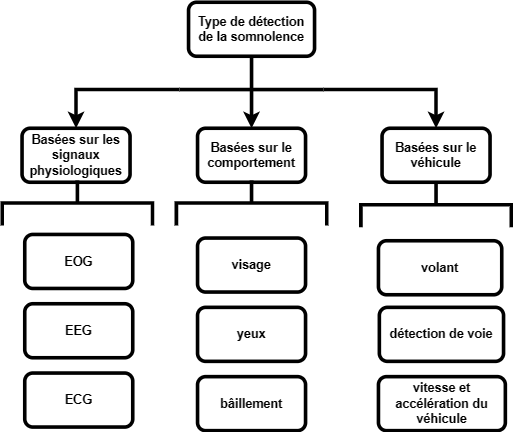
\includegraphics[]{img/indicateurs.drawio.png}
    \caption{ Types  de détection de la somnolence}
     \hypertarget{fig01}{}
\end{figure}
\subsection{Méthodes basées sur des signaux physiologiques}
Ce type de technique repose sur l'exploitation des signaux physiologiques associés à la réponse du corps à la fatigue, à l'aide de capteurs fixés sur le corps du conducteur. Elle utilise des données acquises à partir de capteurs physiologiques tels que l'électrooculographie (EOG), l'électrocardiographie (ECG), l'électroencéphalographie (EEG).

Un électroencéphalographie (EEG) est un examen qui permet de détecter l’activité électrique dans le cerveau à l’aide de petits disques métalliques (électrodes) fixés sur le cuir chevelu (la tête). Les cellules du cerveau transmettent des signaux électriques et sont toujours actives, même lorsque vous dormez. Des lignes ondulées tracent l’activité et sont enregistrées pendant l’EEG. Cet examen permet de diagnostiquer plusieurs troubles du cerveau, notamment l'état de vigilance et les troubles du sommeil\cite{EEG} .

Les chercheurs se concentrent souvent sur des bandes de fréquences telles que les ondes alpha, thêta et delta, où la bande delta (entre 0,5 et 4 Hz) indique l'activité de sommeil, la bande thêta (entre 4 et 8 Hz) indique la somnolence, et la bande alpha (entre 13 et 25 Hz) correspond à la vigilance. L'analyse de l'activité électrique du cerveau fournit des informations sur les états cognitifs et les niveaux de vigilance\cite{sahayadhas2012detecting}.
 
 \begin{figure}[H]
    \centering
    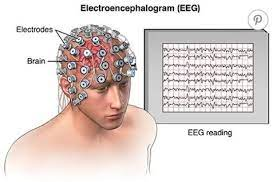
\includegraphics[]{img/EEG.jpg}
    \caption{Placement des électrodes EEG}
     
\end{figure}
L'électrocardiographie ECG est une technique qui repose sur la détection de l'activité électrique du cœur à l'aide d'électrodes placées sur le corps du conducteur. Cet enregistrement peut servir de marqueur potentiel pour prédire la somnolence ou la fatigue en se basant sur la variabilité de la fréquence cardiaque (VFC)\cite{abe2014development,zhang2012drowsiness} . La VFC est un indicateur du fonctionnement du système nerveux autonome (SNA), qui régule les activités cardiaques pour maintenir l'homéostasie du système cardiovasculaire. L'activité du SNA varie selon les périodes de stress, de fatigue et de somnolence. Pendant l'éveil, l'activité sympathique (AS) augmente et/ou l'activité parasympathique (APS) diminue, tandis que pendant la somnolence ou la fatigue, on observe une augmentation de l'APS ou une diminution de l'AS\cite{vicente2011detection}. Différentes méthodes temporelles et fréquentielles ont été utilisées pour analyser la VFC à partir des intervalles RR (IRR),où un IRR  représente le temps qui sépare le début de deux ondes R successives dans le tracé de l’ECG. Les variations de ces caractéristiques temporelles et fréquentielles de l'ECG peuvent fournir des indications sur l'état de somnolence.
 \begin{figure}[H]
    \centering
    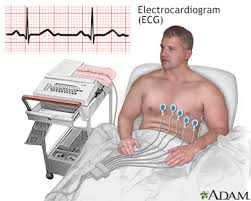
\includegraphics[]{img/ECG.jpg}
    \caption{Placement des électrodes ECG}
     
\end{figure}
L’électrooculographie (EOG) est une technique d’enregistrement des mouvements oculaires en utilisant des électrodes placées autour des yeux. Cette méthode permet de détecter et d’enregistrer les mouvements des yeux, tels que les clignements des yeux et les mouvements lents caractéristiques de la somnolence. En plaçant les électrodes autour des yeux.Le signal EOG identifie la somnolence en se basant sur les mouvements oculaires en mesurant le potentiel électrique entre la cornée et la rétine à partir du champ électrique qui reflète l'orientation de l'œil\cite{sahayadhas2012detecting}.l’EOG mesure les variations du potentiel électrique générées par les mouvements des muscles oculaires. Ces variations sont enregistrées sous forme de signaux électriques qui peuvent être analysés pour évaluer l’activité oculaire et détecter les signes de somnolence chez le conducteur.\\
%Les signaux physiologiques peuvent fournir une mesure précise de la somnolence car ils sont fortement corrélés avec la somnolence. Cependant, cela utilise des techniques invasives et peut rendre le conducteur inconfortable en raison de problèmes de portabilité et de faisabilité limitée\cite{mittal2016head,awais2017hybrid}.%
 

\subsection{Détection  basée  sur le véhicule }
Ce type de détection mesure le niveau de somnolence en fonction des capteurs embarqués dans le véhicule et recueille plusieurs métriques indicatives pour déterminer le niveau de vigilance/somnolence du conducteur grâce à ses comportements de conduite\cite{doudou2020driver}. Les trois principaux aspects de ce type incluent le mouvement du volant, la déviation et la position du véhicule, ainsi que la vitesse et l'accélération du véhicule. L'angle et la trajectoire du volant deviennent irréguliers, et la plage de déviation augmente significativement lorsqu'un conducteur est dans un état de somnolence\cite{dong2010driver,zhong2007localized} . Les approches utilisant la déviation et la position du véhicule reposent sur certaines métriques telles que l'écart-type de la position de la voie (SDLP), qui mesure la position du véhicule par rapport à la voie médiane de la route. Il a été démontré que le score KSS(score de somnolence de Karolinska ) du conducteur peut affecter le score SDLP car les deux sont étroitement liés. Par conséquent, plus le conducteur est somnolent, plus le score SDLP sera élevé, et le SDLP pourrait être un indicateur potentiel pour détecter la somnolence\cite{dong2010driver,chen2015identification,ingre2006subjective}. Enfin, la vitesse et l'accélération du véhicule peuvent indiquer une conduite anormale causée par la somnolence, car les conducteurs somnolents peuvent augmenter ou diminuer accidentellement l'accélération de leur véhicule\cite{doudou2020driver}. 

\subsection{Détection  basée sur le comportement}
Ce type de détection se focalise sur l'analyse des caractéristiques du visage telles que le clignement des yeux, le bâillement et la direction du regard sont capturées à l'aide d'un capteur intégré dans la voiture, puis observées pour détecter la somnolence\cite{vijayan2020comparative} . Les paramètres utilisés dans la détection de la somnolence comprennent le pourcentage de fermeture des yeux (PERCLOS), le rapport d'aspect de l'œil (EAR), le rapport d'aspect de la bouche (MAR) et la position de la tête. Le PERCLOS est le pourcentage du nombre total de trames où les yeux sont détectés comme fermés dans un intervalle de trame spécifique. Un seuil prédéterminé est défini afin de classifier si les yeux sont fermés ou ouverts. Ensuite, le PERCLOS est calculé sur la base de la zone approximative de l'iris pour identifier la somnolence du conducteur\cite{junaedi2018driver,zhang2017research} . Pendant ce temps, l'EAR est utilisé pour enregistrer la fréquence de clignotement des yeux en fonction de la proportion entre la hauteur et la largeur de l'œil\cite{maior2020real,you2019real2,soukupova2016eye} . La valeur EAR est presque constante lorsque l'œil est ouvert et tombe à zéro lorsque l'œil est fermé. Le MAR est similaire à l'EAR, mais il utilise davantage de repères de la bouche pour détecter les bâillements, et l'échelle est opposée à l'EAR. Plus la bouche est ouverte, plus la valeur de MAR sera grande\cite{houssaini2019real,mohanty2019design}. Le MAR peut être mesuré en fonction des régions de couleur rouge des lèvres. Cependant, la performance dépend encore fortement des conditions d'éclairage \cite{niloy2020brief}. Le changement de position de la tête est l'un des phénomènes de comportement typiques montrés par les conducteurs somnolents. Il est généralement observé chez les conducteurs au début de la somnolence, marqué par l'augmentation de la fréquence des inclinaisons de la tête vers l'arrière\cite{brandt2004affordable,dreissig2020driver} .

\subsection{ Comparaison entre les techniques de détection de somnolence }
\begin{table}[htbp]
    \centering
    \begin{tabularx}{\textwidth}{|X|X|X|X|}
    \hline
        techniques  & Mesures & avantages & Incovénients \\
        \hline
      basée sur le comportement& Fermeture des yeux et position de tête, bâillement et analyse de la bouche , l’expression faciale  &  Non-intrusifs, facile à utiliser & Dépend des conditions extérieures\\ 
      \hline
      basée sur me véhicule & Angle du volant, détection de voie et la vitesse de véhicule & Non-intrusifs & Conditions climatiques, l’état des routes, expérience de conducteur\\
      \hline
      basée sur les signaux physiologiques &  ECG, EOG, EEG & Détection anticipée, fiable & Intrusif, faible qualité de signal dans les solutions non-intrusives \\
\hline
    \end{tabularx}
    \caption{Comparaison entre les types des techniques de détection de somnolence}
    \label{tab:my_label}
\end{table}


Voici une version corrigée de votre texte :

Malgré la fiabilité des signaux physiologiques pour la détection de la somnolence, leur intrusivité réside dans la nécessité d'un équipement supplémentaire qui doit être attaché au corps du conducteur pour collecter les données permettant d'identifier son état. De même, les systèmes basés sur le véhicule, qui dépendent de plusieurs paramètres extérieurs, restent des indices difficiles à exploiter et peuvent perturber le conducteur. Cette limitation rend ces deux techniques inappropriées à mettre en œuvre en temps réel. Par conséquent, la plupart des études se concentrent sur la troisième catégorie, qui utilise les caractéristiques comportementales des conducteurs, car elles sont non invasives et impliquent la vision par ordinateur pour la détection de la somnolence. Les mesures comportementales, telles que les mouvements oculaires habituels, les expressions faciales, les bâillements et l'orientation de la tête, sont mesurées sans nécessiter l'ajout d'équipement supplémentaire, sauf une caméra pour capturer les images. En conséquence, l'analyse des caractéristiques comportementales est une solution rentable et facile à utiliser, mais elle reste un défi à améliorer pour une exploitation optimale étant donné la qualité des données acquises.

\section{Approches de détection de la somnolence}
% mena 

Étant donné que la détection de la somnolence basée sur le comportement du conducteur offre des solutions rentables et non intrusives ne nécessitant pas d'équipement supplémentaire, nous avons choisi de mener une recherche sur les solutions déjà adoptées dans ce domaine. Plus particulièrement, celles basées l'apprentissage profond et la vision par ordinateur, en commençant par présenter une étude comparative des travaux déjà réalisés basés sur ces technologies.\\
\begin{table}[htbp]
    \centering
    \begin{tabularx}{\textwidth}{|X|X|X|X|X|}
    \hline
       \textbf{Référence}  & \textbf{Jeu de données} & \textbf{Méthods}&\textbf{Meilleur résultat}& \textbf{Année}\\ \hline
       \cite{chirra2019deep} &Un ensemble de données privé comprend 2850 images & Deep-stacked CNN& Précision de 96,42\% & 2019 \\ \hline
      
        \cite{salman2021driver}&YawDD, qui se compose de 107 images & Ensemble CNN (ECNN) & Score F1 de 93 \%  & 2021\\ \hline
        \cite{rajkar2022driver} & Deux ensembles de données : le Closed Eye in the Wild (CEW) et le Yawing Detection Dataset (YawDD)& réseaux de neurones convolutifs (CNN) & précision de 96.86\% & 2022 \\ \hline
       \cite{Florez2023ACA}  &Ensemble de vidéos NITYMED & InceptionV3, VGG16 et ResNet50V2 &  Précision de 99,71 \% & 2023  \\ \hline
  
    \end{tabularx}
    \caption{Modèles de détection de la somnolence basés sur l'apprentissage profond }
    
    \label{tab:my_label}
\end{table}
\newpage
Dans l'étude \textbf{\cite{chirra2019deep}} ils ont proposé un systeme de détection de la somnolence du conducteur basé sur  l'état des yeux en utilisant l'apprentissage profond. La méthode de détection de visage Viola-Jones est utilisée pour reconnaître la région des yeux, un réseau de neurones convolutifs profonds empilés est créé pour déterminer les images clés importantes dans les séquences de caméra, et la couche SoftMax dans un classificateur CNN est utilisée pour classifier si le conducteur est endormi ou non.  Le travail proposé est évalué sur un ensemble de données collectées et montre une meilleure précision avec 96,42 \% par rapport au CNN traditionnel.\\ \\



Dans l’étude mentionnée dans \textbf{\cite{rajkar2022driver}}, les auteurs ont proposé un système basé sur deux modèles de réseaux de neurones convolutifs (CNN) pour identifier la somnolence du conducteur en utilisant la méthode de la cascade de HAAR pour la détection du visage et des yeux. Le premier modèle CNN a été entraîné et testé sur un ensemble de données CEW pour l'état des yeux, tandis que le deuxième a été entraîné et testé sur le jeu de données YawDD pour détecter l'état de la bouche, qu'elle soit fermée ou ouverte. Les deux modèles ont atteint une précision moyenne de 96,86 \%.\\ \\


Une autre étude \textbf{\cite{salman2021driver}} a proposé un système basé sur quatre techniques différentes de CNN appliquées à l'ensemble de données YawDD pour mesurer le degré de somnolence en fonction de la fréquence des bâillements, des poses spécifiques et des variations d'occlusion. Le réseau de neurones convolutifs ensembliste (ECNN) proposé a surpassé les approches traditionnelles basées sur les CNN, atteignant un impressionnant score F1 de 0,935. Les trois autres approches CNN (CNN1, CNN2 et CNN3) ont obtenu des scores F1 de 0,92, 0,90 et 0,912, respectivement.\\ \\


Dans l’étude mentionnée dans \cite{Florez2023ACA}, Florez et al. ont proposé un système de détection de la somnolence au volant via l’identification en temps réel de l’état des yeux en utilisant trois algorithmes d’apprentissage profond pré-entraînés, à savoir InceptionV3, VGG16 et ResNet50V2. À cet égard, ils ont utilisé l’ensemble de données appelé NITYMED pour l'entraînement, contenant des vidéos de conducteurs présentant divers états de somnolence, où les yeux ont été extraits après la conversion des vidéos en utilisant un algorithme basé sur l'exploitation des points de MediaPipe Mesh. Ce système a été testé sur une partie de test de la même dataset et a atteint une précision de 99,71 \%, marquée par le modèle ResNet50V2 pré-entraîné, démontrant ainsi son efficacité. %

% lahna 


\section{Jeux de données utlisés pour la détection de la somnolence}
\begin{enumerate}
    \item \textbf{YawDD}: est un ensemble de données de détection de l'ouverture de la bouche (ou du sommeil) qui comprend deux jeux de données vidéo de conducteurs avec différentes caractéristiques faciales. Les vidéos ont été recueillies en demandant à des candidats masculins et féminins de s'asseoir dans le siège du conducteur d'une voiture. Les vidéos ont été enregistrées dans des conditions d'éclairage réelles et variables. 
Le premier jeu de données comprend 322 vidéos, où une caméra est installée sous le rétroviseur avant du véhicule. Chaque participant dispose de trois ou quatre vidéos avec différentes conditions de bouche, telles que normale, parlant/chantant et ouvrant la bouche. 

Le deuxième jeu de données comprend 29 vidéos, où une caméra est installée sur le tableau de bord devant le conducteur. Chaque participant dispose d'une seule vidéo avec les mêmes conditions de bouche, toutes dans la même vidéo. Le véhicule était garé pour les deux jeux de données pour assurer la sécurité de l'environnement pour les participants\cite{inproceedings}.
\item \textbf{NITYMED}:Ce jeu de données comprend 130 vidéos capturées à Patras, en Grèce, mettant en scène des conducteurs dans de vraies voitures circulant dans des conditions nocturnes, où détecter la somnolence est particulièrement crucial. Les conducteurs participant à l'ensemble de données se composent de 11 hommes et de 10 femmes, chacun présentant diverses caractéristiques telles que la couleur des cheveux, la présence de barbe et de lunettes. Les vidéos sont divisées en deux catégories principales :

Bâillements : Ces vidéos montrent des conducteurs baillant trois fois par vidéo, chaque vidéo durant environ 15 à 25 secondes. Il y a 107 vidéos dans cette catégorie.

Microsommeils : Dans ces vidéos, les conducteurs s'adonnent à des activités telles que parler et regarder autour d'eux, ponctuées de moments de microsommeil. Chaque vidéo de cette catégorie dure environ 2 minutes, et il y en a 21 disponibles\cite{nitymed}.
\item \textbf{CEW}:  cet ensemble de données contient 2423 sujets, parmi lesquels 1192 sujets avec les deux yeux fermés ont été collectés directement sur Internet, et 1231 sujets avec les yeux ouverts ont été sélectionnés à partir de la base de données LFW\cite{CEW}.
\end{enumerate}
\section{Synthése}
D'après l'examen et la comparaison des travaux déjà existants dans le domaine de la détection de la somnolence , qui se base sur l'analyse du comportement des conducteurs et utilise l'apprentissage profond, nous constatons que la plupart de ces travaux ont opté pour l'utilisation des réseaux de neurones convolutifs (CNN) lors de la conception de leurs modèles. De plus, l'adoption de la notion d'apprentissage par transfert, en exploitant les connaissances des modèles pré-entraînés, ainsi que la combinaison de modèles, a nettement amélioré leurs performances et leur efficacité dans la détection de systèmes déjà existants dans ce domaine. Il est important de noter que le choix du jeu de données a également contribué à cette amélioration de performance et d'efficacité .

\section{l'analyse oculaire pour la détection de la somnolence }
Dans un monde où la fatigue au volant peut avoir des conséquences désastreuses, la technologie d'analyse oculaire associée à la détection de la somnolence représente une avancée significative pour la sécurité routière. Cette technologie innovante utilise des systèmes de suivi oculaire pour analyser les mouvements et les clignements des yeux, permettant ainsi de détecter les premiers signes de somnolence chez les conducteurs. Par exemple, en Europe, cette technologie existe déjà sous la forme d'une option dans les véhicules haut de gamme, appelée DMS (Driver Monitoring System), qui utilise l'intelligence artificielle pour détecter les signes d'endormissement grâce à une caméra embarquée qui filme le visage et détecte les yeux même à travers des lunettes de soleil et dans des conditions d'éclairage ou d'illumination défavorables. Le système est capable de détecter la fermeture ou l'ouverture de la pupille, la fréquence des clignements des yeux et la direction du regard, comme illustré dans la \hyperlink{figDMS}{figure}, afin d'analyser l'état de vigilance du conducteur et d'envoyer ensuite des messages d'avertissement appropriés. Malgré le potentiel de cette technique, elle ne sera implantée que sur les véhicules neufs en Europe\cite{DMS}.
\begin{figure}[htbp]
    \centering
    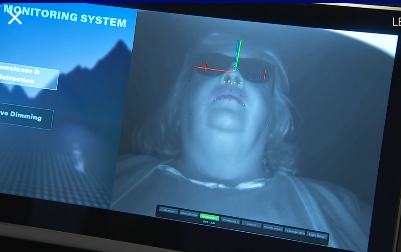
\includegraphics[width=0.5\textwidth ]{img/DMS.png}
    \caption{Driver Monitoring System }
    \hypertarget{figDMS}{}
    
\end{figure}
\subsection{Différence entre le globe oculaire et la région oculaire}
Le terme "oculaire" peut être lié à deux termes différents : "le globe oculaire" et "la région oculaire", qui peuvent être exploités différemment. Nous souhaitons clarifier la distinction entre ces deux termes, étant donné que notre étude se concentrera sur l'analyse de la région oculaire pour la détection de la somnolence.
\begin{enumerate}
    \item \textbf{Globe oculaire}\\
    le globe oculaire est un système (organe) important et interconnecté qui désigne toute la zone de l'œil, y compris le segment antérieur et postérieur de l'œil, et qui inclut généralement, mais sans s'y limiter, tous les tissus fonctionnels (par exemple, pour la vision) ou structuraux présents dans le globe oculaire, ainsi que les tissus ou les couches cellulaires qui tapissent en partie ou en totalité l'intérieur ou l'extérieur du globe oculaire. Les régions oculaires comprennent la chambre antérieur le cristallin, le nerf optique, la hambre postérieure, la cavité vitréenne, la choroïde, l'espace suprachoroïdien, l'espace sous-rétinien, la conjonctive, l'espace sous-conjonctival, l'espace épiscléral, l'espace intracornéen, l'espace épicornéen, la sclérotique, la pars plana, les régions avasculaires induites chirurgicalement, la macula et la rétine\cite{fedorchak2019thermoresponsive}. 
    \item \textbf{Région oculaire}\\
    D'une autre maniere, la région oculaire fait référence à la partie du visage qui contient l’œil et ses environs, tels que les cils, les paupières, les sourcils et la peau autour de l’œil\cite{Vizoni2020OcularRU}. 
\end{enumerate}



\begin{figure}[htbp]
    \centering
    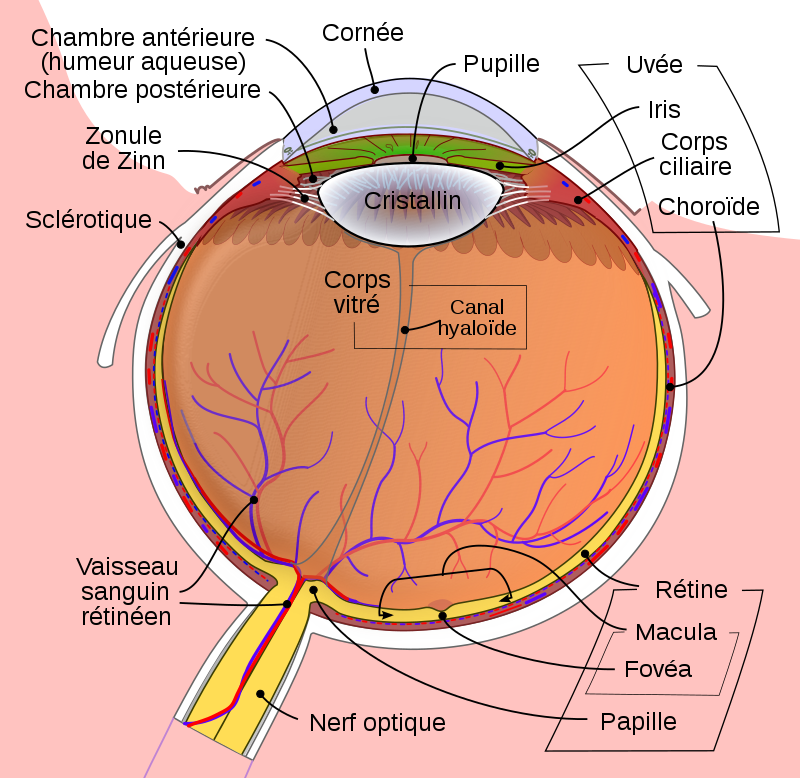
\includegraphics[width=0.5\textwidth ]{img/region_oculaire.png}
    \caption{globe oculaire }
    
\end{figure}
\begin{figure}[htbp]
    \centering
    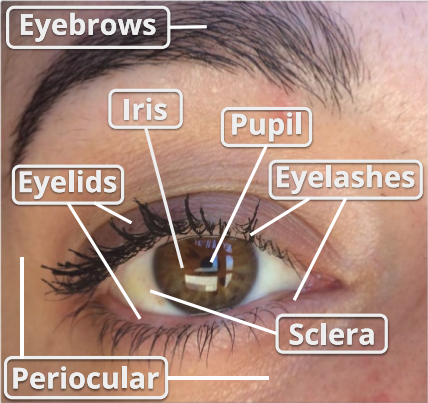
\includegraphics[width=0.5\textwidth ]{img/composants oculaire.png}
    \caption{région oculaire}

\end{figure}

\newpage


\subsection{Étapes de la reconnaissance oculaire}
 En général, la reconnaissance oculaire dédiée à la détection de la somnolence fonctionne selon ces étapes :

\begin{enumerate}
   \item \textbf{Acquisition de l'image}\\
    L'acquisition des données est une étape essentielle dans la reconnaissance oculaire. Les données sont collectées à partir de diverses sources telles que les caméras Pi Cam, les téléphones mobiles ou les caméras de surveillance.
   \item \textbf{Pré-traitement des données}\\
     Une fois que les données sont acquises, elles sont normalisées à une taille et un format spécialisés, puis subissent un pré-traitement afin de réduire le bruit et obtenir une bonne qualité d'image.
   \item \textbf{Détection de visage}\\
   L'étape suivante consiste à localiser le visage dans l'image, dans le but de faciliter la détection de la région oculaire, et ainsi éliminer les parties non pertinentes de l'image.
   \item \textbf{Détection de la région oculaire}\\
   Une fois que le visage est détecté à partir de l'image, il faut ensuite détecter la région d'intérêt qui contient les parties nécessaires de la région oculaire, puis l'identifier et l'isoler.
   \item \textbf{Amélioration de la résolution}\\
   Après la détection de la région de l’œil, l'étape suivante consiste à améliorer la résolution de l'image. Cette étape est appliquée lorsque la qualité de l'image est basse ou lorsque le nombre de pixels est limité.
   \item \textbf{Prétraitement (Alignement du centre de l'œil)}\\
   Après l'amélioration de la résolution de l'image, celle-ci est prétraitée pour aligner le centre de l’œil, ce qui implique d'ajuster l'image pour que le centre de la pupille soit positionné au milieu de l’image. Cela permet ensuite de détecter et d’isoler les parties pertinentes de la région oculaire, telles que l’iris ou la région périoculaire.
   \item \textbf{Extraction des caractéristiques}\\
   Cette étape consiste à identifier et extraire les caractéristiques distinctives de la région oculaire. Cela peut inclure l’analyse des motifs uniques de l’iris, la forme de l’œil et d’autres caractéristiques périoculaires.
   \item \textbf{Comparaison et correspondance}\\
   Enfin, cette étape consiste à comparer les caractéristiques extraites à une base de données de motifs oculaires connus pour trouver une correspondance.
\end{enumerate}



\begin{figure}[htbp]
    \centering
    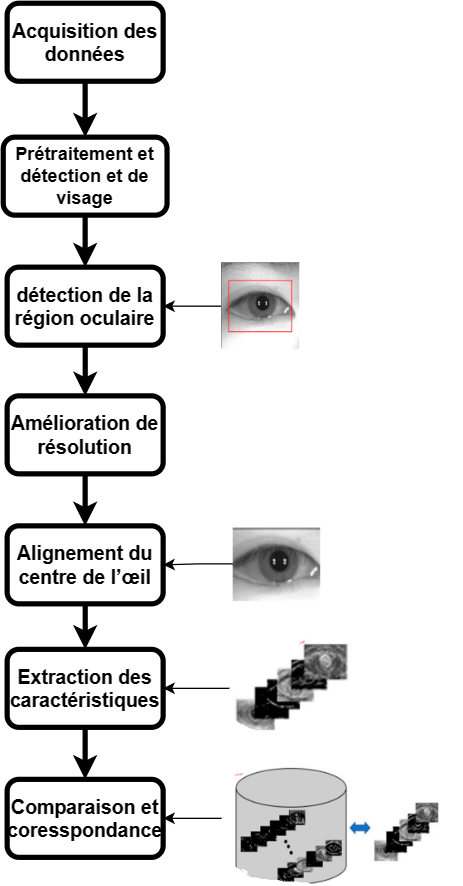
\includegraphics[width=0.5\textwidth ]{img/Diagramme sans nom.drawio.png}
    \caption{étapes de la reconnaissance oculaire}

\end{figure}

\subsection{Autre applications de l'analyse oculaire}
L'analyse oculaire peut non seulement être utilisée dans la détection de la somnolence, mais elle peut etre employé dans d'autres applications dans divers domaines et contextes. Les plus célèbres sont :
\begin{enumerate}
    \item \textbf{L'authentification biométrique}:L’analyse oculaire peut en effet servir à l’identification et la vérification des individus en utilisant les caractéristiques distinctives de leurs yeux. Les principales caractéristiques exploitées sont l’iris, la rétine et la région périoculaire (autour des yeux). Chacune de ces caractéristiques présente des motifs uniques qui peuvent être capturés et analysés pour l’identification.
    \item \textbf{Contrôle d'accès et sécurité }:L’analyse oculaire, attribuée à la reconnaissance oculaire, offre un haut niveau de précision pour distinguer les individus. Cela en fait un outil efficace à adopter dans divers systèmes de sécurité pour la vérification de l’identité, le contrôle d’accès et la surveillance. De même, certains smartphones intègrent la reconnaissance de l’iris pour offrir un déverrouillage sécurisé des appareils mobiles, assurant ainsi la protection des données personnelles et la confidentialité des utilisateurs.
    \item \textbf{Applications médicales et de santé }:Dans le domaine des applications médicales et de santé, les images oculaires sont largement utilisées à des fins diagnostiques et de suivi des maladies oculaires. De plus, la télémédecine bénéficie de la vérification de l'identité des patients lors de consultations à distance, améliorant ainsi l'accessibilité et la qualité des soins.
    \item \textbf{surveillance des conducteurs} :  elle joue un rôle important dans la surveillance des conducteurs, en identifiant les indices de somnolence ou d’inattention et la fatigue,  contribuant ainsi à la sécurité routière.
\end{enumerate}
\section{conclusion}
Durant ce chapitre, nous avons présenté les différents indices les plus utilisés dans les techniques de détection de la somnolence, en mettant en évidence leurs avantages et inconvénients. Nous avons également choisi de présenter des solutions axées sur le comportement du conducteur, notamment celles basées sur l’apprentissage profond, compte tenu de leurs performances remarquables. Nous avons examiné l’impact de l’apprentissage par transfert et de l’apprentissage ensembliste sur l’amélioration des résultats dans la détection de la somnolence. De plus, nous avons mentionné les jeux de données les plus utilisés par ces solutions. Enfin, nous avons défini la reconnaissance oculaire, en détaillant ses étapes et ses applications.













\chapter{Gestion automatisée du stationnement: État de l'art}
\markboth{Gestion automatisée du stationnement: État de l'art}{}

\section{Introduction}
\subsection{ Détection de visage et  localisation des points caractéristiques}
La détection des visages ainsi que des yeux sont deux tâches complexes dans des scénarios réels en raison des variations de posture des conducteurs et des facteurs environnementaux non contrôlés, tels que l’éclairage et l’occlusion. Plusieurs méthodes ont été mises en œuvre pour réaliser cette tâche, parmi les plus utilisées figurent celles basées sur les classificateurs en cascade de Haar, proposées par Paul Viola et Michael Jones en 2001\cite{HaarCascades}. Cette approche repose sur l'apprentissage automatique où une fonction en cascade est entraînée à partir d'un grand nombre d'images positives et négatives, puis utilisée pour détecter des objets dans d'autres images.

MediaPipe Face Mesh, qui est une solution de géométrie faciale qui estime 468 repères 3D du visage en temps réel. Cette solution utilise l’apprentissage automatique (ML) pour inférer la géométrie en 3D de la surface du visage \cite{MediaPipe} afin de repérer les régions d'intérêt tels les yeux.
Cependant, pour notre cas, l'utilisation de la cascade de Haar et de MediaPipe Mesh pour la détection des yeux s'est révélée difficile et peu efficace, contrairement au MTCNN.

En utilisant le cadre multitâche en cascade MTCNN basé sur la profondeur, la détection de visage et l’alignement peuvent être effectués simultanément. La relation interne entre ces deux tâches est exploitée pour améliorer les performances, et les caractéristiques globales du visage sont extraites. Ainsi, les positions du visage, des yeux gauche et droit, peuvent être obtenues. La structure du MTCNN est illustrée dans la \hyperlink{fig3} {figure 1}. Le MTCNN se compose de trois sous-réseaux en cascade : le P-Net (réseau de proposition), le R-Net (réseau affiné) et l’O-Net (réseau de sortie), qui détectent la position du visage et des points caractéristiques de manière progressive et précise.
\begin{figure}[H]
    \hypertarget{fig3}{}
    \centering
    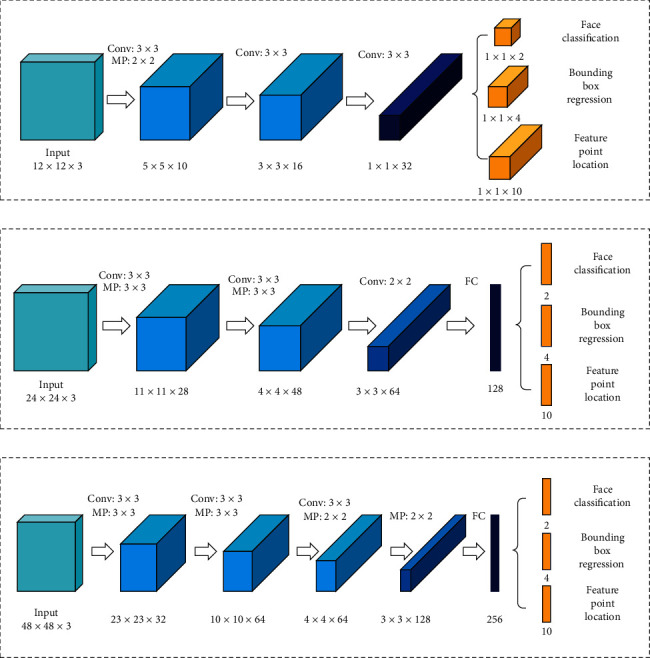
\includegraphics{img/CIN2020-7251280.002.jpg}
    \caption{L'architecture MTCNN : (a) P-Net, (b) R-Net, and (c) O-Net.}
    \label{fig:enter-label}
\end{figure}
\begin{enumerate}
    \item \textbf{}\\
    \item \textbf{}\\
    \item \textbf{}\\
\end{enumerate}

\chapter*{Conclusion générale}
\markboth{Conclusion générale}{}
\addcontentsline{toc}{chapter}{Conclusion générale}
\thispagestyle{plain}
% ------------------------------ new 




\addcontentsline{toc}{chapter}{Bibliographie}
\lhead{}
\rhead{\textit{Bibliographie}}
\nocite{*}
\bibliographystyle{plain}
\bibliography{biblio}

\chapter*{Annexe}
\markboth{Annexe}{}
\addcontentsline{toc}{chapter}{Annexe}
\thispagestyle{plain}



  
  \begin{figure}
  \centering    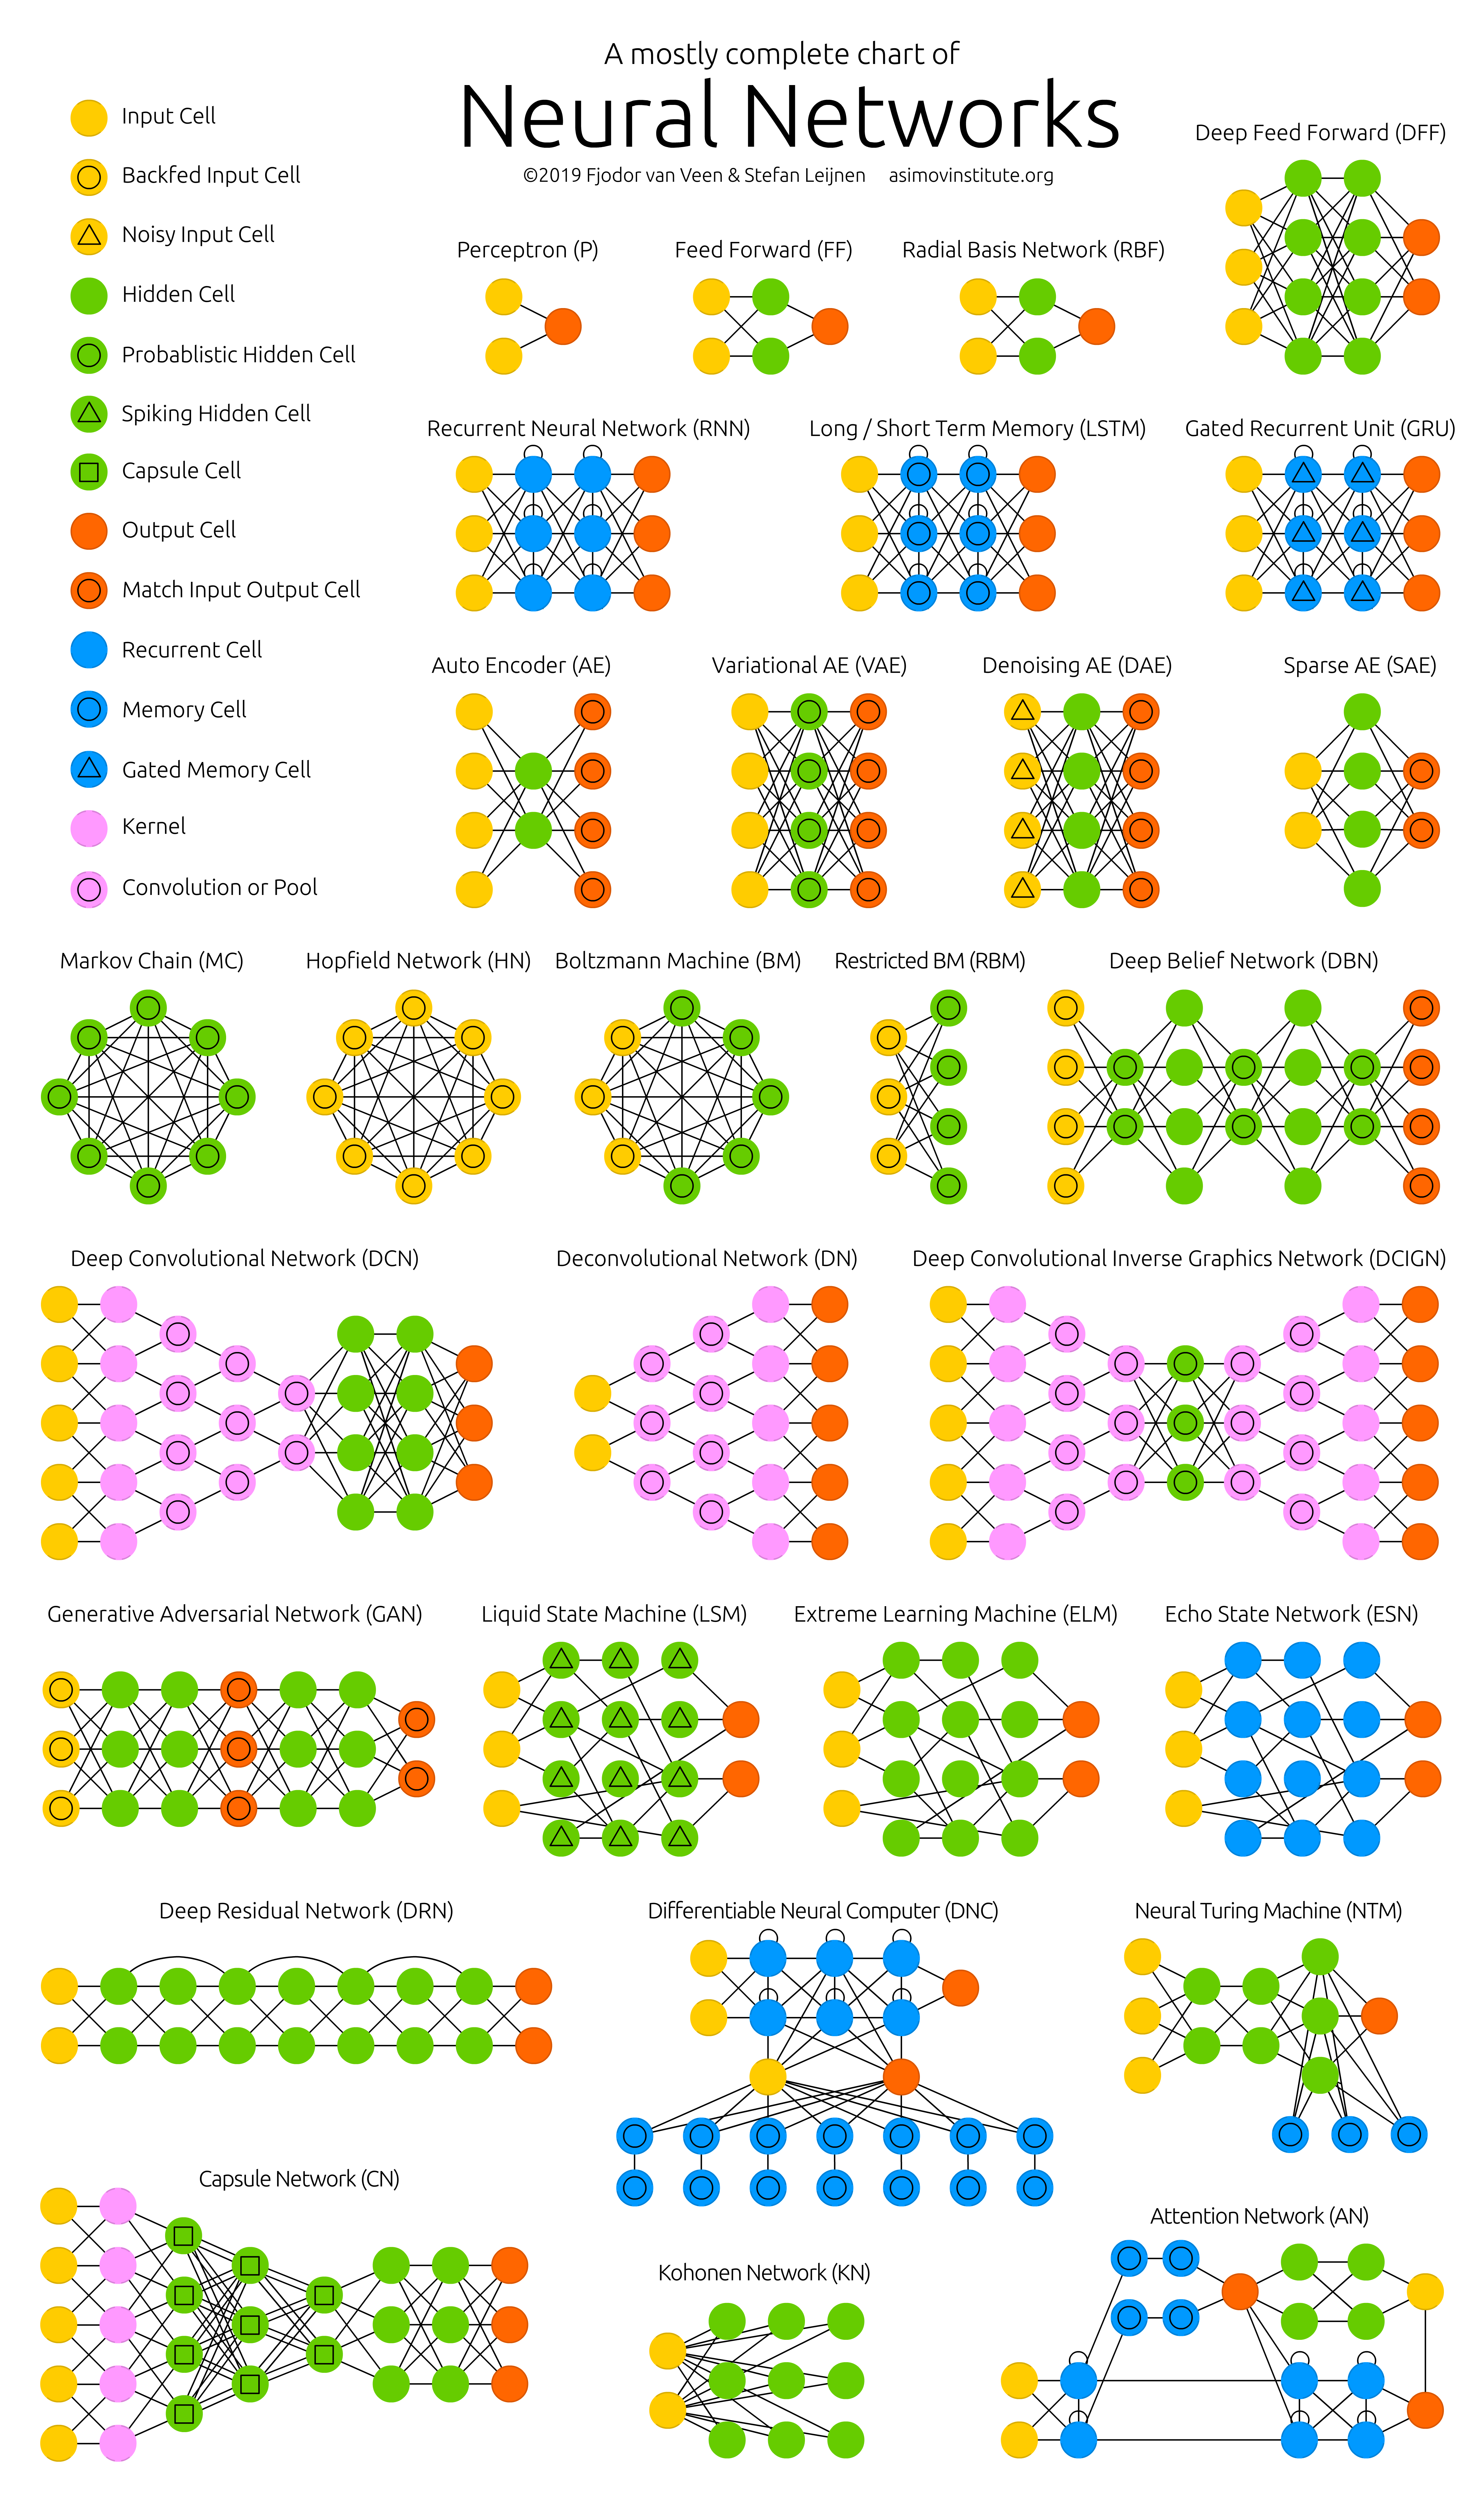
\includegraphics[width=1\textwidth,height=0.95\textheight]{NeuralNetworkZo19High.png}
  \caption{Un aperçu des architectures de réseaux neuronaux\cite{leijnen2020neural}}
  \label{fig:NN_architectures}
  \end{figure}
\end{document}